%% This is a LaTeX template for preparing papers for Publ. Inst. Math.; version January 2016
%% Please delete everything begining with %% (DOUBLE %).

% Submission number:
\documentclass[12pt]{article}
%\tableofcontents
\usepackage[top=2cm,left=2cm,right=2cm,bottom=2cm]{geometry}
\usepackage{amssymb}
\usepackage{amsmath}
% \begin{equation*}
\usepackage{amsopn}
%
\usepackage{mathrsfs}
\usepackage[hyphens]{url} \urlstyle{same}
\usepackage{graphicx} %% Package for inserting illustrations/figures
\usepackage{amsthm}% proof can be used
%% The following packages are useful (you may want to use them):
%\usepackage{refcheck} %% Checks whether enumerated equations are referred to or not.
                       %% Please remove unnecessary numbers.
%\usepackage{cmdtrack} %% Checks whether all author defined macros are used or not
                       %% (see the end of .log file); unused ones should be removed.
%% Both packages have limitations---consult the package documentation.

\def\baselinestretch{1.5}

\theoremstyle{plain}
 \newtheorem{thm}{\textbf{Theorem}}
 \newtheorem{prop}{Proposition}[section]
 \newtheorem{lem}{\textbf{Lemma}}
 \newtheorem{cor}{\textbf{Corollary}}
\theoremstyle{definition}
 \newtheorem{exm}{\textbf{Example}}
 \newtheorem{dfn}{\textbf{Definition}}
\theoremstyle{remark}
 \newtheorem{rem}{\textbf{Remark}}

%% Please, do not change the following four lines:
\renewcommand{\le}{\leqslant}\renewcommand{\leq}{\leqslant}
\renewcommand{\ge}{\geqslant}\renewcommand{\geq}{\geqslant}
\renewcommand{\setminus}{\smallsetminus}

%% Please use the newest classification -- 2010
%% available at  http://msc2010.org/MSC-2010-server.html
%% and the newest amsproc.cls.
%% Please, classify to the third level,
%% e.g., 26A and 26Axx are not satisfsctory.

%%\keywords{optional, but desirable}

%% OTHER AUTHOR(S):
%\author[]{}
%\address{ }
%\email{}

%\thanks{Supported by ... } %% optional
%\thanks{Communicated by ...} %% This will be filled in the journal office.
\begin{document}

\begin{titlepage}
   \begin{center}
       \vspace*{1cm}

       \textbf{\large Empirical Spectral Distributions for Products of Rectangular Matrices}

       \vspace{0.5cm}


       \vspace{1.5cm}

       \textbf{A PROJECT \\ SUBMITTED TO THE FACULTY OF THE GRADUATE SCHOOL\\ OF THE UNIVERSITY OF MINNESOTA\\ BY }\\
        \vspace{1 cm}
        \textbf{Hongru Zhao}\\

       \vspace{1cm}
       \textbf{IN PARTIAL FULFILLMENT OF THE REQUIREMENTS\\ FOR THE DEGREE OF\\ Master of Science}
       \vspace{1 cm}

       \vspace{1 cm}
       \textbf{Advisor: Dr. Yongcheng Qi}
       \\
        \vspace{1 cm}
        \textbf{\today}
   \end{center}
\end{titlepage}




%\author{Hongru Zhao}
%\address{ %% Put here your affiliation; street address is not required
%   Department of Mathematics and Statistics \\ % \hfill (Received 00 00 201?)\\
%   University of Minnesota Duluth   \\ %\hfill (Revised  00 00 201?)\\
%   US}
%\email{zhao1118@d.umn.edu}
%{\begin{flushleft}\baselineskip9pt\scriptsize
%PUBLICATIONS DE L'INSTITUT MATH\'EMATIQUE\newline
%Nouvelle s\'erie, tome ??(1??)) (201?), od--do \hfill DOI: \\
%\end{flushleft}}
%\vspace{18mm} \setcounter{page}{1} %\thispagestyle{empty}


\begin{abstract}
Consider a sequence of square matrices, each square matrix is a
product of independent rectangular complex Ginibre ensemble. The
entries of Ginibre ensemble are independent and identically
distributed standard complex Gaussian random variables. In this
paper, our aim is to study the limiting spectral empirical
distributions of the sequence of products. The length of each
product may vary. A complete description for the limiting empirical
spectral distributions is given. Some
examples are presented as well. 

\noindent {\bf Keywords:} Empirical spectral distribution, Product
of rectangular complex Ginibre ensemble, Non-Hermitian random matrix
\end{abstract}


\newpage
\tableofcontents

\newpage



\section{Introduction}\label{sec:intro}
Historically, Random Matrix Theory was discussed by Wishart~\cite{wishart} for statistical analysis of large samples.
Wigner found applications for random Hermitian matrix in nuclear
physics. Based on on Wigner's work, Dyson~\cite{Dyson} found out that
there are three natural classes: real symmetric, complex Hermitian
and real quaternion self-dual. Similarly, Ginibre ensembles of
non-symmetric real, non-Hermitian complex and non-self-dual real
quaternion matrices with Gaussian entries were discussed in
\cite{Ginibre}, which match Dyson indices.

The classical semi-circular law was first introduced by Wigner, and
then Ginibre~\cite{Ginibre} established the circle law for Ginibre
ensembles. Since then, the assumptions were relaxed subsequently in
the papers by Girko~\cite{Girko},  Bai~\cite{Bai},  Pan and
Zhou~\cite{Pan}, and Gotze and Tikhomirov~\cite{GF-TA}. Tao and
Vu~\cite{Tao} proved the circular law under the weakest condition.

Products of random matrices are particularly of interest in recent
research. Ipsen~\cite{Ipsen} provides several applications,
including wireless telecommunication, disordered spin chain, the
stability of large complex system, quantum transport in disordered
wires and so on. Two recent papers by Jiang and
Qi~\cite{JiangQi2019, 2017} consider the spectral radii and limiting
empirical spectral distribution. Then Qi and Xie~\cite{SRP} found
the limiting spectral radii for rectangular products.

In this paper, we consider the product of $m$ random rectangular
matrices with independent and identically distributed (i.i.d.)
complex Gaussian entries and investigate the limiting distributions
for the empirical spectral distribution. When length of each product ensemble is fixed integer,
Zeng~\cite{zeng2016} obtained the limiting empirical spectral
distribution. When these rectangular matrices are actually squared
ones, the product matrix is reduced to the product of Ginibre
ensembles, which has been studied in Jiang and
Qi~\cite{JiangQi2019}.


\section{Main Results}\label{sec:main}
%In this paper we will study the limiting spectral laws of one type of random matrices.
In this paper, we consider $m$ independent rectangular matrices, $\mathbf{X}_j$, $1\leq j \leq m$, namely each $\mathbf{X}_j$ is an $n_j\times n_{j+1}$, matrix for $1\leq j\leq m$, where $n_1,\cdots, n_{m+1}$ are positive integers, and all entries of the $m$ matrices are independent and identically distributed (i.i.d.) standard complex normal random variables. We assume $n_1=n_{m+1}=:n$ so that the product, $\mathbf{X}=\mathbf{X}_1 \cdots \mathbf{X}_{m}$ is an $n\times n$ square matrix. Assume $m$ depends on $n$, i.e. $m=m_n$. We also assume $n=\min_{1\leq j\leq m+1}n_j$. In this case the product matrix $\mathbf{X}$ is of full rank. Our results hold for any positive integer $m$, which may depend on $n$.

Denote the $n$ eigenvalues of $\mathbf{X}$ as $\mathbf{z}_{1},
\cdots, \mathbf{z}_{n}$, and set $l_{j}=n_{j}-n\geq 0$, $j=1,
\cdots, m$. It follows from Theorem 2 of Adhikari et
al.~\cite{Adhikari} that the joint density function for
$\mathbf{z}_{1}, \cdots, \mathbf{z}_{n}$ is given by
\begin{equation*}
p\left({z}_{1}, \cdots, {z}_{n}\right)=C \prod_{1 \leq j<k \leq
n}\left|{z}_{j}-{z}_{k}\right|^{2} \prod_{j=1}^{n}
w_{m}^{\left(l_{1}, \cdots,
l_{m}\right)}\left(\left|z_{j}\right|\right)
\end{equation*}
with
respect to the Lebesgue measure on $\mathbb{C}^{n}$, where $C$ is a
normalizing constant such that $p(z_1,\cdots, z_n)$ is a probability
density function, and function $w_{m}^{\left(l_{1}, \cdots,
l_{m}\right)}(z)$ can be obtained recursively by
\begin{equation*}
w_{k}^{\left(l_{1}, \cdots, l_{k}\right)}(z)=2 \pi \int_{0}^{\infty}
w_{k-1}^{\left(l_{1}, \cdots,
l_{k-1}\right)}\left(\frac{z}{s}\right)
w_{1}^{\left(l_{k}\right)}(s) \frac{d s}{s}, \quad k \geq 2
\end{equation*} with initial $w_{1}^{(l)}(z)=\exp
\left(-|z|^{2}\right)|z|^{2 l}$ for any $z$ in the complex plane,
see Zeng~\cite{zeng2016}.

Our objective in the paper is to investigate the limiting empirical
spectral distribution of the product ensemble $\mathbf{X}$ when $n$
tend to infinity. We allow $m$ change with $n$ and write $m=m_n$ to
show its dependence of $n$.


The empirical spectral distribution of $\mathbf{X}$ is the empirical distribution based on the eigenvalue of $\mathbf{X}$ as $\mathbf{z}_{1}, \cdots, \mathbf{z}_{n}$, i.e.,
\begin{equation}\label{equ:mu*}
\mu^*_n=\frac{1}{n}\sum_{j=1}^n \delta_{\mathbf{z}_j/a_n},
\end{equation}
where $a_n>0$ is a sequence of normalizing constants. In this paper,
$m$ can change with $n$. When $m=m_n$ diverges with $n$, the
maginitude of $\mathbf{z}$'s can go to infinity exponentially or
vanish exponentially. In this case, one may not be able to find a
sequence $a_n$ such that the empirical measure $\mu_n^*$ converges.
Instead, we will define empirical distribution for scaled
eigenvalues as in Jiang and Qi ~\cite{JiangQi2019}.

Note that $\{ \mathbf{z}_j;1\leq j\leq n \}$ are complex random variables. Write
$$
\Theta_j=\arg(\mathbf{z}_j)\in[0,2\pi), \text{ such that }\mathbf{z}_j=|\mathbf{z}_j|e^{i\Theta_j},
$$
for $1\leq j\leq n$. Further, assume that $Y_1,\cdots,Y_n$ are independent random variables, and random variable $Y_j$ has a density function proportional to $y^{j-1}w_m^{(l_1,l_2,\cdots,l_m)}(y)I(y>0)$. Given a sequence of measurable functions $h_n(r)$, $n\geq 1$, defined on $(0,\infty)$, set
\begin{equation}\label{equ:mun}
\mu_{n}=\frac{1}{n} \sum_{j=1}^{n} \delta_{\left(\Theta_{j}, h_{n}\left(\left|\mathbf{z}_{j}\right|\right)\right)} \text { and } \nu_{n}=\frac{1}{n} \sum_{j=1}^{n} \delta_{h_{n}\left({Y_{j}}\right)},
\end{equation}

We will see later that the convergence of $\mu_n$ is closely related to that of $v_n$. In (\ref{equ:mun}), if $h_n$ is linear, that is $h_n(r)=r/a_n$, where $\{ a_n,n\geq 1 \}$ is a sequence of positive numbers, we denote the empirical measure of $\mathbf{z}_j$'s by $\mu_n^*$ as in (\ref{equ:mu*}), and accordingly, we denote the empirical distribution $Y_j$'s by
$$
\nu_n^*=\frac{1}{n} \sum_{j=1}^{n} \delta_{{Y_{j}}/a_n}.
$$
Notation:
\begin{itemize}
    \item Any function $g(z)$ of complex variable $z=x+iy$ should be interpreted as a bivariate function of $(x,y):g(z)=g(x,y)$.
    \item We write $\int_Ag(z)dz=\int_Ag(x,y)dxdy$ for any measurable set $A\subset \mathbb{C}$.
    \item \text{Unif}($A$) stands for the uniform distribution on a set $A$.
    \item For a sequence of random probability measures $\{ \tau,\tau_n;n\geq 1 \}$, we write
    \begin{equation}\label{equ:leadsto converge}
    \tau_{n} \leadsto \tau \text { if } \mathbb{P}\left(\tau_{n} \text { converges weakly to } \tau \text { as } n \rightarrow \infty\right)=1
    \end{equation}
\end{itemize}

When $\tau$ is a non-random probability measure generated by random variable $X$, we simply write $\tau_n\leadsto X$.

Review the notation "$\leadsto$" in (\ref{equ:leadsto converge}).
The symbol $\mu_1\otimes \mu_2$ represents the product measure of two measures $\mu_1$ and $\mu_2$.

We first cite Theorem 1 in Jiang and Qi ~\cite{JiangQi2019} as
follows.

\begin{thm}\label{thm:nonlinear}
Let $\phi(x)\geq 0$ be a measurable function define on $[0,\infty)$. Assume the density of $(z_1,\cdots,z_n)\in \mathbb{C}^n$ is proportional to $$\prod_{1\leq j<k\leq n} |z_j-z_k|^2\prod_{j=1}^n\phi (|z_j|).$$
Let $Y_1,\cdots,Y_n$ be independent r.v.'s such that the density of $Y_j$ is proportional to $y^{2j-1}\phi(y)I(y\geq 0)$ for every $1\leq j\leq n$. If $\{ h_n \}$ are measurable functions such that $\nu_n\leadsto \nu$ for some probability measure $\nu$, then $\mu_n\leadsto \mu$ with $\mu=\text{Unif}[0,2\pi]\otimes \nu$.

Taking $h_n(r)=r/a_n$, the conclusion still holds if "$(\mu_n$,$\nu_n$,$\mu$,$\nu)$" is replaced by "$(\mu_n^*$,$\nu_n^*$,$\mu^*$,$\nu^*)$" where $\mu^*$ is the distribution of $Re^{i\Theta}$ with $(\Theta,R)$ having the law of $\text{Unif}[0,2\pi]\otimes \nu^*$.
\end{thm}
It follows from Theorem \ref{thm:nonlinear} that a common feature for limiting empirical distributions from determinant point processes that the angle and radius of the random vector with the liming distribution are independent.

Inspired by Jiang and Qi ~\cite{JiangQi2019}, and Zeng
~\cite{zeng2016}, we define the following sequence of functions
$F_n(x)$ and generalize their ideas for our theorem \ref{thm:main
theorem} and theorem \ref{thm: ln F(x) limit}. The limiting spectral
distribution actually depends on the limit of functions $F_n(x)$ as
defined below. Let $\left\{\gamma_{n} ;  n \geq 1\right\}$ be a
sequence of positive numbers. Define 
\begin{equation}
    \label{equ:F_n}
    F_{n}(x)=\left(\prod_{j=1}^{m_n} \frac{nx+l_{j} }{n+l_{j}}\right)^{1 / \gamma_{n}}=
    \left(\prod_{j=1}^{m_n} (1-\frac{n}{n_j}(1-x))\right) ^{1 / \gamma_{n}},  x \in[0,1]
\end{equation}
The sequence  $\gamma_{n}$ is called scale sequence.
Note that $F_n(x)$ are continuous and strictly increasing on $[0,1]$, $F_{n}(0)=0$ and $F_{n}(1)=1$. We will assume that $F_n(x)$ converges weakly to a distribution function $F(x)$ such that $F(0-)=0, F(1)=1$.

%\begin{rem}\label{Kn F(x)}If $\exists n_j<n_1$, then let $K_n=min\{ n_j : 1\leq j\leq m_n\}$, and define\begin{equation*}F_n(x)= \left(\prod_{j=1}^{m_n} (1-\frac{K_n}{n_j}(1-x))\right) ^{1 / \gamma_{n}},  x \in[0,1]\end{equation*}\end{rem}

%Assume that $F_n(x)$ converges weakly to a distribution function $F(x)$. We assume $1\leq\gamma_{n}\leq m_n$ without loss of generality.  
We will first determine the types of the limit $F$ and then reveal the relationship between the limit $F$ and limiting empirical spectral distribution (limit measure of $\mu_n$).


% In Section~\ref{sec: a study in gamma}, we will show that  $F(x)$ can only be of the type of one of the three classes in Theorem
%\ref{thm:classification}.


\subsection{Structures of limit function $F(x)$}

%%Now our aim is to find the properties of the limiting function $F(x)$.
Firstly, the classification theorem for limiting distribution $F(x)$
is as follows.

\begin{thm}\label{thm:classification}
    Let $m=m_n$ be a sequence of positive integers. If $F_n(x)$ converges weakly to a distribution function $F(x)$, then $F$ is of the type of one of the following three classes:
    \begin{itemize}
    \item[(i).] $F(x)$ is continuous and strictly increasing on $[0,1]$, $F(0+)\geq0$ and
    $F(1)=1$;

    \item[(ii).] $F(0-)=0$, $F(x)=1$ for all $x\in [0,1]$;

    \item[(iii).] $F(1)=1$, $F(x)=0$ for all $x\in [0,1)$ .
    \end{itemize}
    Moreover,  we have
\begin{itemize}
\item[(a).] $F(x)$ is of class (ii) if and only if there exists $x\in
(0,1)$ such that $F(x)=1$ if and only if
    \begin{equation*}
    \frac{1}{\gamma_{n}} \sum_{r=1}^{m} \frac{n}{n+l_{r}} \rightarrow 0.
    \end{equation*}
\item[(b).]
    $F(x)$ is of class (iii) if and only if there exists $x\in (0,1)$ such that $F(x)=0$ if and only if
    \begin{equation*}
    \frac{1}{\gamma_{n}} \sum_{r=1}^{m} \frac{n}{n+l_{r}} \rightarrow
    \infty.
    \end{equation*}
\item[(c).]
    $F(x)$ is of class (i) if and only if there exists $x\in (0,1)$ such that $F(x)\in (0,1)$, which implies
    there exists constant $c_1$ and $c_2$ such that
    \begin{equation}
    0<c_{1} \leqslant \frac{1}{\gamma_{n}} \sum_{r=1}^{m} \frac{n}{n+l_{r}} \leqslant c_{2}<\infty.
    \end{equation}
\end{itemize}
\end{thm}









\begin{thm}\label{thm:Newclassification}
    Let $m_n$ be a sequence of positive integers, and $\gamma_n$ be arbitrary sequence of positive numbers. 
    Then there exists a subsequence $n_s$, such that $F_{n_s}(x)$ converges weakly to a distribution function $F(x)$, and $F$ is of the type of one of the following three classes:
    \begin{itemize}
    \item[(i).] $F(1)=1$, $F(x)=0$ for all $x\in [0,1)$;
    
    \item[(ii).] $F(0-)=0$, $F(x)=1$ for all $x\in [0,1]$;
    
    \item[(iii).] $F(x)$ is continuous on $[0,1]$, and analytic on $(0,1)$, with $F(0+)\geq0$, 
    $F(1)=1$, and $F'(x)> 0 ,x\in (0,1)$ .
    \end{itemize}
    With loss of generality, we use $n$ to denote the subsequence $n_s$. Three classes of limiting distributions have the following characteristic. 
\begin{itemize}
\item[(a).] $F_n(x)$ convergence weakly to class (i) limit, if and only if 
    \begin{equation*}
    \frac{1}{\gamma_{n}} \sum_{r=1}^{m_n} \frac{n}{n_{r}} \rightarrow \infty,
    \end{equation*}
\item[(b).]
    $F_n(x)$ convergence weakly to class (ii) limit  if and only if
    \begin{equation*}
    \frac{1}{\gamma_{n}} \sum_{r=1}^{m_n} \frac{n}{n_{r}} \rightarrow
    0,
    \end{equation*}
\item[(c).]
    $F_n(x)$ convergence weakly to class (iii) limit, if and only if  for all positive integer $k$, 
    \begin{equation}
     \lim_{n\rightarrow\infty}\frac{1}{\gamma_{n}} \sum_{r=1}^{m_n} \left(\frac{n}{n_{r}}\right)^k
    \end{equation}
    exist, and there exists positive $c_1$, $c_2$ such that
    \begin{equation}
    0< c_1\leq\frac{1}{\gamma_{n}} \sum_{r=1}^{m_n} \frac{n}{n_{r}}\leq c_2<\infty. \end{equation}
\end{itemize}
\end{thm}


\begin{proof}
    First of all, we set $$g_n(x)=\ln(F_n(x))\leq 0,x\in(0,1], \text{ and }a_k{(n)}=\frac{1}{\gamma_{n}} \sum_{r=1}^{m_n} \left(\frac{n}{n_{r}}\right)^k.$$
    Easy to check $0<a_k{(n)}\leq a_k{(1)},\forall k\geq 1$.
    
    Employing Taylor expansion $\ln(1-t)=-\sum_{k\geq 1} \dfrac{t^k}{k},|t|<1$, we have for $x\in(0,1]$ 
    \begin{equation*}
    g_n(x)=-\sum_{k=1}^\infty \frac{a_k{(n)}}{k}(1-x)^k.
    \end{equation*}
    
    Fixed $ 0<\delta<1$, $\forall z$ such that $|z-1|\leq \delta$, we have
\begin{equation}\label{equ:uniformly bounded}
     \sum_{k=1}^\infty \left|-\frac{a_k{(n)}}{k}(1-z)^k\right|\leq \sum_{k=1}^\infty \frac{a_k{(n)}}{k}\delta^k=|g_n(1-\delta)|<\infty.
\end{equation}
    
    Thus, we could extent $g_n(x)$ to be a complex analytic function on disk $D=\{z\in\mathbb{C};|z-1|<1\}$, namely
    \begin{equation}\label{equ:taylor g_n(x)}
    g_n(z)=-\sum_{k=1}^\infty \frac{a_k{(n)}}{k}(1-z)^k.
    \end{equation}

    The following inequality is useful,
    \begin{align}    &a_1{(n)}(1-x)\leq-g_{n}(x)\leq a_1{(n)}\sum_{k=1}^\infty \frac{1}{k}(1-x)^k =a_1{(n)}\times (-\ln (1-x)),x\in(0,1);\label{ine:useful inequality}
    %&\frac{-g_n(y)}{-\ln(1-y)}\leq a_1(n)\leq \frac{-g_n(y)}{1-y},y\in(0,1)\label{ine:useful inequality2}.
    \end{align}


\textbf{Claim1: }For any sequence of positive numbers $\gamma_n$, there exists a subsequence $n_s$, such that $F_{n_s}$ converges weakly to $F(x)$, and $F(x)$ is of the type of one of the three classes.

\textbf{Birth of three classes:}

    \textbf{Case 1:} There exists $0<x_0<1$ such that $g_n(x_0)$ is unbounded.
    
    Thus, there exists a subsequence $n_s$ such that $g_{n_s}(x_0)\rightarrow -\infty$, which implies $a_1{(n_s)}\rightarrow \infty$ as $s\rightarrow \infty$, by using inequality (\ref{ine:useful inequality}). Then fixed $x\in(0,1)$, employing inequality (\ref{ine:useful inequality}) again, we have $-g_{n_s}(x)\rightarrow \infty$ i.e. $F(x)=\lim_{s\rightarrow\infty}\exp\{g_{n_s}(x)\}=0$. Hence $F(x)$ is of class (i).
    
    \textbf{Case 2:} Suppose for all $0<x<1$, $g_n(x)$ is bounded, and there exists $0<x_0<1$ and a subsequence $n_s$ such that $g_{n_s}(x_0)\rightarrow0$.
    
    Then inequality (\ref{ine:useful inequality}) forces $a_1{(n_s)}\rightarrow 0$, as $s\rightarrow \infty$.
    
    Similar to previous discussion, fixed $x\in(0,1)$, we have $g_{n_s}(x)\rightarrow 0$.
    
    Hence $F(x)=\lim_{s\rightarrow\infty}\exp\{g_{n_s}(x)\}=1,x\in (0,1)$, which is of class $(ii)$.
    
    \textbf{Case 3:} Suppose for each $x\in (0,1)$ 
    $$
    -\infty<\inf_{n} g_{n}(x)\leq \sup_{n} g_{n}(x)<0.
    $$
    Similar to previous discussion, we know 
    $a_1{(n)}(1-x)\leq-g_{n}(x)\leq a_1{(n)}(-\ln(1-x))$.
    Hence there exists positive $c_1$ and $c_2$ such that $0<c_1\leq a_1^{(n)}\leq c_2<\infty,\forall n$.
    
    Now we aim to use Montel's theorem to find a subsequence $n_s$ such that $g_n(z)$ converges uniformly on each compact subsets of $D=\{z\in\mathbb{C};|z-1|<1\}$.
    
In ~\cite{RudinComplex}, theorem 14.6 is so called
\textbf{Montel's theorem}.
Suppose $f_n(z)$ is a sequence of analytic functions on open set $\Omega\subset\mathbb{C}$. If $f_n(z)$ is uniformly bounded on each compact subset of the region $\Omega$, then there exists a subsequence $f_{n_s}$, which converges uniformly on each compact subsets of $\Omega$, i.e. there exists a analytic function $f$ on $\Omega$, such that $f_{n_s}$ converges uniformly to $f$ on each compact subsets of $\Omega$.

For each $\delta\in(0,1)$, $z\in K_\delta:=\{z\in D;|z-1|\leq\delta\}$ \begin{equation*}
    |g_n(z)|=| \sum_{k=1}^\infty \frac{a_k{(n)}}{k}(1-z)^k|\leq \sum_{k=1}^\infty \frac{a_k{(n)}}{k}|1-z|^k\leq \sum_{k=1}^\infty \frac{a_k{(n)}}{k}\delta^k=|g_n(1-\delta)|<\infty.
\end{equation*}

Thus, $g_n(z)$ is uniformly bounded on $K_\delta=\{z\in D;|z-1|\leq\delta\}$.

There exists a analytic function $g(z)$ on $D$, such that $g_{n_s}$ converges uniformly to $g$ on each compact subsets of $D$. 

The uniform convergence on compact subsets arises most naturally in connection with limit operations on analytic function in the following sense.

\textbf{Theorem 10.28 in ~\cite{RudinComplex}}: Suppose $f_j$ is analytic on open set $\Omega\subset \mathbb{C}$, for $j=1,2,\cdots,$ and $f_j\rightarrow f$ uniformly on each compact subsets of $\Omega$. Then $f$ is analytic on $\Omega$, and $f'_j\rightarrow f'$ uniformly on compact subsets on $\Omega$.


Thus, for $k$-th order derivetive, we have $g_{n_s}^{(k)}(1)\rightarrow g^{(k)}(1)$ as $s\rightarrow \infty$, i.e. 
\begin{align*}
    &a_{1}{(n_s)}\rightarrow a_1 \in [c_1,c_2], \text{ as } s\rightarrow \infty,\\
    &a_{k}{(n_s)}\rightarrow a_k \in [0,\infty),k\geq 2, \text{ as } s\rightarrow \infty,\\
    &\text{where }g(z)=-\sum_{k=1}^\infty \frac{a_k}{k}(1-z)^k.
\end{align*}
Hence $g'(x)=\sum a_k (1-x)^{k-1}>0, x\in (0,1)$.

Set $F(x)=e^{g(x)},0<x\leq 1$. It is easy to verify $F(1)=1$ ,$ F_n(x)>0$, $F_n(x)=e^{g_{n_s}(x)}\rightarrow F(x)$ pointwise and $F'(x)=F(x)g'(x)>0$ for fixed $x\in(0,1)$. Hence $F_{n_s}$ converges weakly to a distribution function $F(x)$, and $F(x)$ is analytic on $(0,1)$. That is the birth of class $(iii)$ limit.

Hence, we finish the proof of claim 1.

\textbf{Claim 2:} If the subsequence $F_{n_s}(x)$ convergence weakly to a distribution function $F(x)$, then $F(x)$ must be of the type of one of the previous three classes.

View $F_{n_s}(x)$ as our original sequence, by similar discussion, we know that there exists a new subsequence $n_{s_{j}}$, such that $F_{n_{s_j}}(x)$ convergence weakly to $G(x)$, which is of type of one of the previous three classes. Since weak limit is unique, we have $F(x)=G(x)$. 

Hence, we finish the proof of claim 2.




\textbf{Proof of statement (a):}
    Assume $a_1{(n)}\rightarrow \infty$ as $n\rightarrow \infty$. Then fixed $x\in(0,1)$, employing inequality (\ref{ine:useful inequality}), we have $-g_{n}(x)\rightarrow \infty$ i.e. $F(x)=\lim_{n\rightarrow\infty}\exp\{g_{n}(x)\}=0$. Thus, $F(x)$ is of class (i).
    
    Conversely, suppose $F(x)$ is of class (i). Fixed $x_0\in (0,1)$, $F_{n}$ converges weakly to $F$, which implies $g_{n}(x_0)=\ln(F_{n}(x_0))\rightarrow -\infty$. Then, inequality (\ref{ine:useful inequality}) implies $a_1{(n)}\rightarrow \infty$.

\textbf{Proof of statement (b):}
Proof of case $(b)$ is similar to that of case $(a)$. We omit the proof. 

\textbf{Proof of statement (c):}
%Hence, we need to prove case $(c)$. The proof of the sufficient condition is similar to the proof in case 3. We only prove the necessary part.
Assume, 
\begin{equation}
     \lim_{n\rightarrow\infty}\frac{1}{\gamma_{n}} \sum_{r=1}^{m_n} \left(\frac{n}{n_{r}}\right)^k=a_k
    \end{equation}
    exist for $k\geq 1$, and there exists positive $c_1$, $c_2$ such that
    \begin{equation}
    0< c_1\leq\frac{1}{\gamma_{n}} \sum_{r=1}^{m_n} \frac{n}{n_{r}}\leq c_2<\infty. \end{equation}
Notice that $a_{k+1}{(n)}\leq a_k{(n)}$, implies $a_{k+1}\leq a_k\leq a_1$.

Set $g(z)=-\sum_{k=1}^\infty \frac{a_k}{k}(1-z)^k$. The radius of convergence of $g(z)$ satisfies 
$$
R=\frac{1}{\limsup_{n\rightarrow \infty} \left( \frac{a_k}{k}\right)^{1/k} }\geq\frac{1}{\limsup_{n\rightarrow \infty} \left( \frac{a_1}{k}\right)^{1/k} } =1,
$$
i.e. $g(z)$ is well defined on disk $D=\{z\in\mathbb{C};|z-1|<1\}$. 
For each $\delta\in(0,1)$, we claim that $g_n(z)$ is uniformly converges to $g(z)$ on $K_\delta=\{z\in D;|z-1|\leq\delta\}$.
\begin{align*}
    |g_n(z)-g(z)|\leq \sum_{k=1}^N\frac{|a_k{(n)}-a_k|}{k}\delta^k+2\sum_{k=N+1}^\infty \frac{c_2}{k}\delta^k \leq \sum_{k=1}^N|a_k{(n)}-a_k|+\frac{2c_2}{1-\delta}\delta^{N+1}.
\end{align*}

Thus,
\begin{align*}
\limsup_{n\rightarrow \infty}|g_n(z)-g(z)|&=\limsup_{N\rightarrow \infty}\limsup_{n\rightarrow \infty}|g_n(z)-g(z)|\\
&\leq \limsup_{N\rightarrow \infty}\limsup_{n\rightarrow \infty}
\sum_{k=1}^N|a_k{(n)}-a_k|+\frac{2c_2}{1-\delta}\delta^{N+1}\\
&\leq   \limsup_{N\rightarrow \infty}\frac{2c_2}{1-\delta}\delta^{N+1}=0.
\end{align*}
 
Set $F(x)=e^{g(x)},0<x\leq 1$. 

Similar to the discussion in case 3, we have
$F_n(x)=e^{g_{n_s}(x)}\rightarrow F(x)$ pointwise on $(0,1)$, $F(1)=1$, $ F_n(x)>0$, and $F'(x)=F(x)g'(x)>0$ for fixed $x\in(0,1)$. Thus, $F(x)$ is a distribution function restrict to $(0,1]$, and $F(x)$ is analytic on $(0,1)$. So $F$ is of class (iii).

Hence $F_{n}$ converges weakly to distribution function $F(x)$.

Now, we assume $F_n(x)$ converges weakly to $F(x)$, which is of class (iii). 

Set $g_n(x)=\ln (F_n(x))$. Since each $x\in (0,1)$, 
$-\infty<\inf_{n} g_{n}(x)\leq \sup_{n} g_{n}(x)<0,$
then proof of case 3 implies there exists a subsequence $n_s$, such that $F_{n_s}(x)$ converges weakly to a class (iii) limit $F(x)=e^{g(x)},x\in (0,1)$, and
\begin{align*}
    &a_{1}{(n_s)}\rightarrow a_1 \in (0,\infty), \text{ as } s\rightarrow \infty,\\
    &a_{k}{(n_s)}\rightarrow a_k \in [0,\infty),k\geq 2, \text{ as } s\rightarrow \infty,\\
    &\text{where }g(z)=-\sum_{k=1}^\infty \frac{a_k}{k}(1-z)^k.
\end{align*}
%and $g_{n_{s}}(z)\rightarrow g(z)$ uniformly on each compact subsets of $D$. 


Suppose the following conditions fail for some $k$,
\begin{align*}
    &a_{1}{(n)}\rightarrow a_1 \in (0,\infty), \text{ as } n\rightarrow \infty,\\
    &a_{k}{(n)}\rightarrow a_k \in [0,\infty),k\geq 2, \text{ as } n\rightarrow \infty.
\end{align*}

\textbf{Case $\alpha$:}
Suppose there exists $n_j$ such that $a_1(n_j)\rightarrow \infty$.

Statement $(a)$ implies $F_{n_j}(x)=e^{g_{n_j}(x)}\rightarrow0,x\in (0,1)$, which is not of class $(iii)$. 
Hence we obtain a contradiction.

\textbf{Case $\beta$:}
Suppose $c_2:=\sup a_1(n)<\infty$. Then $a_k(n)\leq a_1(n)\leq c_2$. Assume there exists a subsequence such that $a_1(n_j)\rightarrow 0$.

Statement $(b)$ implies $F_{n_j}(x)=e^{g_{n_j}(x)}\rightarrow 1,x\in (0,1)$, which is not of class $(iii)$. 
Hence we obtain another contradiction.

\textbf{Case $\gamma$:}
Suppose $a_k(n)\leq c_2<\infty,\forall k\geq 1$, and $\inf_n a_1(n)>0$. Assume there exists a $k$ and another subsequence $n_j$, such that $a_k(n_j)\rightarrow a_k^*\neq a_k$.

The simply diagonal argument for a sequence of bounded sequences $\{a_{k'}(n)\}_{n=1}^\infty$ implies there exists a subsequence $n_{j_t}$ and some numbers $a_{k'}^*,k'\geq 1, k'\neq k $ such that 
\begin{align*}
    &a_{1}{(n_{j_t})}\rightarrow a_1^* \in (0,\infty), \text{ as } t\rightarrow \infty,\\
    &a_{k}{(n_{j_t})}\rightarrow a_k^* \in [0,\infty),k\geq 2, \text{ as } t\rightarrow \infty.
\end{align*}
Set $g^*(z)=-\sum_{k=1}^\infty \frac{a_k^*}{k}(1-z)^k$. 

As we discussed before, we know that $g_{n_{j_t}}(z)\rightarrow g^*(z)$ uniformly on each compact subsets of $D$. 

Since the weak limit is unique, we obtain $g(x)=g^*(x),x\in (0,1)$. Since $x=1$ is removable discontinuity for both $g$ and $g^*$, we could view $g(x)=g^*(x),x\in (0,1]$. Hence, $g^{(k)}_-(1)=g^{*(k)}_-(1)$, i.e. $a_k=a_k^*$, which contradicts our assumption $a_k\neq a_k^*$.

We finish the proof.

\end{proof}







\begin{rem}\label{stange}
    Even though $F_n(0)=0$, it is still possible that $F(0+)>0$. For instance, let $\gamma_{n}=m_n\to \infty$, $ l_1=0$ and $l_r=n,2\leq r\leq m$, then $F(x)=\frac{x+1}{2}, x\in (0,1)$.
\end{rem}

\begin{lem}\label{lem:necessary condition for the first class}
Suppose $F_n$, which is defined in equation (\ref{equ:F_n}), with a sequence $\gamma_n$, converges weakly to a distribution function $F(x)$, which is of class (i), then there exists a constant $0<c^*<\infty$ such that
$$\frac{1}{\gamma_n}\sum_{r=1}^{m_n}\frac{n}{n_r}\rightarrow c^* .$$
Moreover, \begin{equation*}
    F^{*}(x)=\left\{\begin{array}{cc}{0,} & {x < F(0)} \\ {F^{-1}(x),} & {x \in[F(0),1)} \\ {1,} & {x \geq 1}\end{array}\right.
    \end{equation*}
is absolutely continues and $F_-'(1)=c^*$, where $F_-'$ denote left derivative of function $F$.



\end{lem}
\begin{rem}
If there exists a sequence $\gamma_n$ such that $F_n(x)$ convergence weakly to a distribution function, which is of class $(i)$, set $\gamma_n=\sum_{r=1}^{m_n}\frac{n}{n_r}$, and define the corresponding $F_n$. Then the new function sequence $F_n(x)$ converges weakly to a class $(i)$ distribution function $F(x)$, such that $F'_-(1)=1$. 

Here, extra condition $F'_-(1)=1$ is used to normalize the limiting distribution $F(x)$, which uniquely determine the class (i) limiting distribution $F(x)$.

Since $1\leq\sum_{r=1}^{m_n}\frac{n}{n_r}\leq m_n$, we could always assume $1\leq \gamma_n\leq m_n$ without loss of generality.
\end{rem}

\begin{rem}
	In practice, we often set $\gamma_{n}=1$,	$\gamma_{n}=m$ or 
	\begin{equation*}
	\gamma_{n}=\sum_{r=1}^{m} \frac{n}{n+l_{r}}.
	\end{equation*}
	Detailedly, if $\sum_{r=1}^{m_n}\frac{n}{n_r}$ converges to a finite constant, then we prefer to set $\gamma_n=1$; if $\frac{1}{m_n}\sum_{r=1}^{m_n}\frac{n}{n_r}$ converges to a positive constant $c\in (0,1]$, then we prefer to set $\gamma_n=m_n$; otherwise we set $\gamma_n=\sum_{r=1}^{m_n}\frac{n}{n_r}$.
\end{rem}


\subsection{Limiting empirical spectral distributions}

\begin{thm}\label{thm:main theorem}
    Let $\{m_n\geq 1;n\geq 1\}$ be an arbitrary sequence of integers. Let $X_1X_2\cdots X_{m_n}$ be a sequence of products of rectangular complex Ginibre ensembles, which follows previous definition.\\

   \noindent (a). Suppose that $F(x)$ is of class $(i)$  with $1\leq\gamma_n\leq m_n$, define
    \begin{equation*}
    F^{*}(x)=\left\{\begin{array}{cc}{0,} & {x < F(0)} \\ {F^{-1}(x),} & {x \in[F(0),1)} \\ {1,} & {x \geq 1}\end{array}\right.
    \end{equation*}
    and define $h_n(x)=\frac{1}{a_n}|x|^{2/\gamma_{n}}$ , where $a_n=\prod_{r=1}^{m_n}n_r^{1/\gamma_{n}}$. Let $\nu$ be a probability measure, which can be determined by $\nu((-\infty,x])=F^*(x)$. Define empirical spectral measure as follows:
    \begin{equation*}
    \mu_{n}=\frac{1}{n} \sum_{j=1}^{n} \delta_{({\arg} (z_{j}), h_n(\left|z_{j}\right|))},
    \end{equation*}
    where  $\delta_{(\Theta,R)}$ is the delta function at $(\Theta,R)$ in polar coordinates.\\
    Then $\mu_{n}$ converges weakly to$\text { Unif }[0,2 \pi) \otimes \nu$ as $n\to
    \infty$.\\

     \noindent (b). Suppose that $F(x)$ is of class $(ii)$ with $1\leq\gamma_n\leq m_n$, define
    \begin{equation*}
    F^{*}(x)=\left\{\begin{array}{cc}{0,} & {x < 1} \\ {1,} & {x \geq 1}\end{array}\right.
    \end{equation*}
    and $h_n(x)=\frac{1}{a_n}|x|^{2/\gamma_{n}}$, where $a_n=\prod_{r=1}^{m_n}n_r^{1/\gamma_{n}}$.
    
    Then $\mu_{n}$ converges weakly to$\text { Unif }\{|z|=1\}$ as $n\to \infty$.\\
Notice that weak convergence in polar coordinates is equivalent to that in Cartesian coordinates.
\end{thm}


%\begin{rem}\label{rem: discard eigenvalue}    Let $K_n=min\{ n_j : 1\leq j\leq m_n\}$. If $n_1>K_n $, then there are $n_1-K_n$ trivial zero eigenvalues for product ensembles. Let $K_n=n_J$. It is trivial that $X_{1} \cdots X_{m_n}$ and $X_{n_J} \cdots X_{m_n} X_{1} \cdots X_{n_{J+1}}$ have exactly the same eigenvalues counting multiplicity except for 0 eigenvalue, we can generalize Theorem \ref{thm:main theorem},  replacing $n$ by $K_n$ and assume that $K_n\rightarrow \infty$ when sequence index $n\rightarrow \infty$.\end{rem}


%By Theorem \ref{thm:main theorem} and Remark \ref{rem: discard eigenvalue}, we obtain the next Corollary.
%\begin{cor}    Let $K_n=min\{ n_j : 1\leq j\leq m_n\}$,  $K_n/n\rightarrow p\in (0,1]$. Suppose $F_n(x)$, which is defined in Remark \ref{Kn F(x)}, converge weakly to a limiting distribution function $F(x)$, then $\mu_{n}$ converge weakly to a probability measure $\text {Unif }[0,2 \pi) \otimes v$, where $v((-\infty,x])=pF^*(x)+(1-p)\delta_0(x)$.\end{cor}


\begin{rem}
By lemma \ref{lem:necessary condition for the first class}, we can define $f^*(r)=\dfrac{d F^*(r)}{dr}, r\in (0,1)$. Then Theorem \ref{thm:main theorem} implies $\mu_{n}=\frac{1}{n} \sum_{j=1}^{n} \delta_{\left(\Theta_{j}, h_{n}\left(\left|z_{j}\right|\right)\right)}$ converges weakly to measure $\mu$ whose density function is given by $p(z)=\frac{1}{2 \pi|z|} f^{*}(|z|)$.
\end{rem}




%Define
%\begin{equation*}
%\mu_{n}=\frac{1}{n} \sum_{j=1}^{n} \delta_{h_n\left(\mathbf{z_{j}}\right)}
%\end{equation*}
%which is the empirical measure of the eigenvalues  $\mathbf{z}_{1}, \cdots, \mathbf{z}_{n}$.
 \noindent



\section{Proofs}

\subsection{Lemmas from previous work}
By Lemma 2.2 and 2.3 from Zeng ~\cite{zeng2017}, let
%Assume $Y_{1}, \ldots, Y_{n}$ are independent random variables such that the density of $Y_j$ is proportional to $y^{2 j-1} w_{m}^{\left(l_{1}, \ldots, l_{m}\right)}(y) I_{y>0}$. By Lemma 1.1 from Jiang and Qi ~\cite{2017} for any %symmetric $n$ function $g\left(t_{1}, \dots, t_{n}\right)$.\\

\begin{equation*}
T_{j}=\prod_{r=1}^{m_n} s_{j, r}, \quad 1 \leq j \leq n,
\end{equation*}
where $s_{j,r}$ follows a Gamma($l_r+j$,1) distribution for any $1 \leq j \leq n, 1 \leq r \leq m_n$, i.e. the density function of $s_{j,r}$ is given by $y^{l_{r}+j-1} e^{-y} I_{y>0} / \Gamma\left(l_{r}+j\right)$.\\



\begin{lem}\label{lem: Zeng 2017   lem 2.3}~\cite{zeng2017}
For $x \in[0, \infty)$,
\begin{equation*}
\mathbb{P}\left(T_{1} \leq x\right) \geq \mathbb{P}\left(T_{2} \leq x\right) \geq \cdots   \geq \mathbb{P}\left(T_{n} \leq x\right)
\end{equation*}
\end{lem}
\begin{lem}\label{lem: Zeng2017 Lemma 2.2}~\cite{zeng2017}
$g\left(T_{1}, \cdots, T_{n}\right)$ and $g\left(\left|z_{1}\right|^{2}, \cdots,\left|z_{n}\right|^{2}\right)$ have the same distribution, for any symmetric function $g(t_1,\cdots,t_n)$.
\end{lem}

Given a sequence of measurable functions $h_{n}(r), n\geq 1$ defined on $[0, \infty)$, set
\begin{equation*}
\mu_{n}=\frac{1}{n} \sum_{j=1}^{n} \delta_{\left(\Theta_{j}, h_{n}\left(\left|z_{j}\right|\right)\right)} \text { and } \nu_{n}=\frac{1}{n} \sum_{j=1}^{n} \delta_{h_{n}\left(\sqrt{T_{j}}\right)},
\end{equation*}
where $\Theta_{j}=\arg \left(z_{j}\right) \in[0,2 \pi)$.\\


By lemma  \ref{lem: Zeng2017 Lemma 2.2}, and Theorem
\ref{thm:nonlinear} from Jiang and Qi ~\cite{JiangQi2019}, we obtain
the lemma as follows.
\begin{lem}\label{lem: Zeng 2017   lem ?}
If {$h_n$} are measurable functions such that  $\nu_{n}$ converges weakly to $v$ for some probability measure $\nu$, then $\mu_{n}$ converge to $\mu$ weakly with $\mu=\text { Unif }[0,2 \pi] \otimes \nu$.
\end{lem}

The following theorem play a significant role to prove Theorem
\ref{thm:main theorem}. The proof is similar to Lemma 2.3 from Zeng
~\cite{zeng2017}.

\begin{thm}\label{thm: ln F(x) limit}
    If $1\leq\gamma_{n}\leq  m_n$ and limiting function $F(x)$ exists, which is not of class $(iii)$, then the following limit holds:
    \begin{equation}
    \frac{1}{\gamma_{n}} \ln \frac{T_{[\mathrm{nx}]}}{\prod_{r=1}^{m_n}(l_r+n)}-\ln F(x) \stackrel{P}{\rightarrow} 0, \quad x \in[0,1]
    \end{equation}
\end{thm}




\subsection{Proofs of Theorem \ref{thm:classification} , \ref{thm: ln F(x) limit} and \ref{thm:main theorem}}
\ \\
    First of all, we start with a trivial inequality, which is formula $(2.44)$ from Jiang and Qi ~\cite{JiangQi2019}.
    \begin{equation} \label{inequality}
    -\frac{1+\delta}{2 \delta}(1-t) \leq \ln t \leq-(1-t) \text { for } \delta \leq t \leq 1
    \end{equation}
\begin{prop}
    Let $m:=m_n$. For fixed $x_0\in (0,1)$,
the following three conditions are equivalent:
\begin{eqnarray*}
&&(a) -\dfrac{1}{\gamma_{n}}\sum_{r=1}^{m}\ln(\dfrac{nx_0+l_r}{n+l_r})\to 0,\\
&&(b) \dfrac{1}{\gamma_{n}}\sum_{r=1}^{m}\dfrac{n}{n+l_r}\to 0,\\
&&(c)-\dfrac{1}{\gamma_{n}}\sum_{r=1}^{m}\ln(\dfrac{nx+l_r}{n+l_r})\to 0, for\ all\ x\in (0,1).
\end{eqnarray*}
\end{prop}
\begin{proof}
Let $t=\dfrac{nx+l_r}{n+l_r}$, then $1-t=\dfrac{(1-x)n}{n+l_r}$ and $x\leq \dfrac{nx+l_r}{n+l_r}\leq 1$.\\
We obtain
\begin{equation}\label{ineq}
-\frac{1+x}{2 x}\dfrac{1}{\gamma_{n}}\sum_{r=1}^{m}\dfrac{(1-x)n}{n+l_r} \leq  \dfrac{1}{\gamma_{n}}\sum_{r=1}^{m}\ln(\dfrac{nx+l_r}{n+l_r}) \leq-\dfrac{1}{\gamma_{n}}\sum_{r=1}^{m}\dfrac{(1-x)n}{n+l_r}
\end{equation}
Hence $(a)\Rightarrow (b)\Rightarrow (c)\Rightarrow (a)$.
\end{proof}
\begin{prop}
    Let $m:=m_n$. For fixed $0<x_1<x_2<1$,
    the following three conditions are equivalent to the previous three conditions:
\begin{eqnarray*}
&&(d) -[\dfrac{1}{\gamma_{n}}\sum_{r=1}^{m}\ln(\dfrac{nx_1+l_r}{n+l_r})-\dfrac{1}{\gamma_{n}}\sum_{r=1}^{m}\ln(\dfrac{nx_2+l_r}{n+l_r})]=-\dfrac{1}{\gamma_{n}}\sum_{r=1}^{m}\ln(\dfrac{nx_2\frac{x_1}{x_2}+l_r}{nx_2+l_r})\to 0,\\
&&(e) \dfrac{1}{\gamma_{n}}\sum_{r=1}^{m}\dfrac{nx_2}{nx_2+l_r}\to 0,\\
&&(f) \dfrac{1}{\gamma_{n}}\sum_{r=1}^{m}\dfrac{nx}{nx+l_r}\to 0, for\ all\ x\in (0,1).
\end{eqnarray*}
\end{prop}
\begin{proof}
    The proof of $(d)\Leftrightarrow(e)$ is similar to the proof of $(a)\Leftrightarrow(b)$. \\
    Since
    \begin{equation*}
x\dfrac{n}{n+l_r}\leq \dfrac{xn}{nx+l_r}\leq \dfrac{n}{n+l_r},
    \end{equation*}
we know $(e)\Rightarrow (b)\Rightarrow (f)\Rightarrow (e)$
\end{proof}
\begin{rem}\label{rem6}
    We can replace property "$\to 0$", by "$\to \infty$"  or  "$\in [c_1,c_2] $, where exists constants $c_1>0, c_2<\infty$", but the constants maybe different under different conditions. Using "$\to 0$" and "$\to \infty$" version equivalence between $(a)$ and $(c)$, we obtain the following corollary.
\end{rem}
\begin{cor}\label{corollary1}
If there exists $x_0\in (0,1)$, such that $F(x_0)=0$, then $F(x)$ is of class $(iii)$.
\end{cor}
\begin{cor}
    If there exists $x_0\in (0,1)$, such that $F(x_0)=1$, then $F(x)$ is of class $(ii)$.
\end{cor}

\begin{lem}\label{lem4_new}
    If there exists $0<x'_{1}<x'_{2}<1$ such that $F(x'_1)=F(x'_2)\neq 0$, then $F(x)$ is of class $(ii)$.
\end{lem}
\begin{rem}\label{rem7_new}
    If $F(x'_1)=F(x'_2)=0$, by corollary \ref{corollary1}, we know that $F(x)$ is of class $(iii)$.\\
\end{rem}
\begin{proof}[\textit{\textbf{Proof of Lemma \ref{lem4_new}}}]
    By squeeze theorem, $F(x)$ exists and takes a constant value on $(x_1',x_2')$. Thus $F(x)$  is continuous at $x_1,x_2$, where $x_1'<x_1<x_2<x_2'$. We know that condition $(d)$ holds. Because of the equivalency between $(d)$ and $(c)$, we obtain that $F(x)=1$ for all $x \in(0,1)$.
\end{proof}
\begin{lem}
If there exists $x_0\in (0,1)$, such that $0<F(x_0)<1$ and weak limit $F(x)$ exists, then $F(x)$ is of class $(i)$.
\end{lem}

\begin{proof}[\textit{\textbf{Proof of Theorem \ref{thm:classification}}}]
    Let $m:=m_n$. By lemma \ref{lem4_new} and remark \ref{rem7_new}, $0<F(x_0)<1$ implies $F(x)$ strictly increasing on $(0,1)$. Using remark \ref{rem6} of proposition, we know that
    \begin{equation*}
    0<c_1\leq \frac{1}{\gamma_{n}} \sum_{r=1}^{m} \frac{n}{n+l_{r}} %\leq \dfrac{m}{\gamma_{n}}\ \ \text {and}\ \% \frac{1}{\gamma_{n}} \sum_{r=1}^{m} \frac{n}{n+l_{r}}
    \leq c_2<\infty.
    \end{equation*}
     We need to prove the continuity of $F(x)$ at $(0,1)$ as well as left continuity at $1$.\\
     Since $F(x)$ is strictly increasing, set of points where $F(x)$ is not continuous is at most countable, which means we can always find a continuous point on any open set.\\
%    First of all, let a sequence $x_k\to 0$ which belongs to the set of points where $F(x)$ is continuous over $(0,1)$.
%\begin{eqnarray*}
%   &&\ \ \frac{1}{\gamma_{n}} \sum_{r=1}^{m} \ln \left(\frac{n x_k+l_{r}}{n+l_{r}}\right)\\
%   &&= \frac{1}{\gamma_{n}} \sum_{r=2}^{m} \ln \left(\frac{n x_k+l_{r}}{n+l_{r}}\right)+
%   \dfrac{1}{\gamma_{n}} ln\ x_k\\
%   &&\leq \dfrac{m}{\gamma_{n}} ln\ x_k\\
%   &&\leq c_1 \  ln\ x_k \to -\infty.
%\end{eqnarray*}
%Hence we obtain $F(x_k)\to 0$, i.e. $F(x)$ is right continuous at 0.\\
First of all, let a sequence $x_k\to 1$ which belongs to the set of point where $F(x_k)$ is continuous over $(0,1)$.
\begin{equation*}
 \frac{1}{\gamma_{n}} \sum_{r=1}^{m} \ln \left(\frac{n x_k+l_{r}}{n+l_{r}}\right)\geq -\frac{1+x_k}{2 x_k} \frac{1}{\gamma_{n}} \sum_{r=1}^{m} \frac{(1-x_k) n}{n+l_{r}} \geq -\frac{(1+x_k)(1-x_k)}{2x_k}c_2\to 0.
\end{equation*}
Hence we get $F(x_k)\to 1$, i.e. $F(x)$ is left continuous at 1.\\
Next, for fixed $x\in (0,1)$, we can still find two sequences of points, such that $x_k\nearrow x$, $y_k\searrow x$ and $F(x)$ is continuous at $x_k$ and $y_k$ for all $k$.\\
We want to proof $F(x_k)-F(y_k)\to 0$, when $x_k\nearrow x$ and $y_k\searrow x$.
\begin{align*}
    0&\geq F(x_k)-F(y_k)\\
  &= \lim _{n \rightarrow \infty} \frac{1}{\gamma_{n}} \sum_{r=1}^{m} \ln \left(\frac{n y_{k} \frac{x_{k}}{y_{k}}+l_{r}}{n y_{k}+l_{r}}\right)\\
  &\geq   -\frac{(1+\frac{x_{k}}{y_{k}})(1-\frac{x_{k}}{y_{k}})}{2 \frac{x_{k}}{y_{k}}} \limsup _{n \rightarrow \infty} \frac{1}{\gamma_{n}} \sum_{r=1}^{m} \frac{ ny_k}{ny_k+l_{r}}\\ &\geq-\frac{\left(1+\frac{x_{k}}{y_{k}}\right)\left(1-\frac{x_{k}}{y_{k}}\right)}{2 \frac{x_{k}}{y_{k}}} c_2\to 0, k\to  \infty
\end{align*}

Hence $F(x)$ is continuous over $(0,1]$. This complete the proof of Theorem \ref{thm:classification}
\end{proof}

\begin{proof}[\textbf{Proof of lemma \ref{lem:necessary condition for the first class}}]Suppose 
$$
F^{\gamma_n}_{n}(x)=\left(\prod_{j=1}^{m_n} \frac{nx+l_{j} }{n+l_{j}}\right)^{1 / \gamma_{n}}=
    \left(\prod_{j=1}^{m_n} (1-\frac{n}{n_j}(1-x))\right) ^{1 / \gamma_{n}},  x \in[0,1].    
$$    
and denote the class $(i)$ weak limit by $F^{\gamma_n}(x)$. Set $\gamma_n'=\sum_{r=1}^{m_n}\frac{n}{n_r}$. Then we could similarly define the corresponding sequence $F^{\gamma_n'}_{n}(x)$.

From theorem \ref{thm:classification}, $F^{\gamma_n}(x)$ is of class $(i)$, which implies $0<c_1\leq\frac{\gamma_n'}{\gamma_n}\leq c_2<\infty$, where $c_1$ and $c_2$ are positive constant.

Hence there exists a positive constant $c^*\in [c_1,c_2]$ and a subsequence $n_j$ such that $\frac{\gamma_{n_j}'}{\gamma_{n_j}}\rightarrow c^*$.

Then 
\begin{align*}
    F^{\gamma_{n_j}'}_{n_j}(x)=(F^{\gamma_{n_j}}_{n_j}(x))^{\frac{\gamma_{n_j}}{\gamma_{n_j}'}}\rightarrow (F^{\gamma_n}(x))^{1/c^*}=:F^{\gamma_{n_j}'}(x),j\rightarrow \infty.
\end{align*}

Now we aim to prove that $(F^{\gamma_{n_j}'})_-'(1)=1$, i.e. the left derivative exists at $1$, and its value is also $1$.

We only need to prove 
$$
\lim_{x\rightarrow 1^-}\lim_{j\rightarrow \infty}\frac{F^{\gamma'_{n_j}}_{n_j}(x)-F^{\gamma'_{n_j}}_{n_j}(x)}{x-1} \text{ exists.}
$$

By mean value theorem, there exists a $\xi_j\in (x,1)$ such that
$$
\frac{F^{\gamma'_{n_j}}_{n_j}(x)-F^{\gamma'_{n_j}}_{n_j}(x)}{x-1}=F^{\gamma'_{n_j}}_{n_j}(\xi_j)\frac{1}{\gamma'_{n_j}}\sum_{r=1}^{m_n}\frac{n}{n\xi_j +l_r}.
$$

By using simple inequalities, we obtain
$$
F^{\gamma'_{n_j}}_{n_j}(x)\leq F^{\gamma'_{n_j}}_{n_j}(x)\frac{1}{\gamma'_{n_j}}\sum_{r=1}^{m_n}\frac{n}{n +l_r}\leq F^{\gamma'_{n_j}}_{n_j}(\xi_j)\frac{1}{\gamma'_{n_j}}\sum_{r=1}^{m_n}\frac{n}{n\xi_j +l_r}\leq \frac{1}{\gamma'_{n_j}}\sum_{r=1}^{m_n}\frac{n}{n x +l_r}\leq \frac{1}{x}.
$$

Let $j\rightarrow \infty$, we obtain 
$$
\limsup_{x\rightarrow 1^-}\limsup_{j\rightarrow \infty}\frac{F^{\gamma'_{n_j}}_{n_j}(x)-F^{\gamma'_{n_j}}_{n_j}(x)}{x-1} \leq 1,
$$
and $F^{\gamma_n}(x)$ is of class $(i)$ implies
$$
\liminf_{x\rightarrow 1^-}\liminf_{j\rightarrow \infty}\frac{F^{\gamma'_{n_j}}_{n_j}(x)-F^{\gamma'_{n_j}}_{n_j}(x)}{x-1} \geq \liminf_{x\rightarrow 1^-}(F^{\gamma_n}(x))^{1/c^*}=1.
$$
Hence $(F^{\gamma_{n_j}'})_-'(1)=1$, which also implies $(F^{\gamma_{n_j}})_-'(1)$ exists and $(F^{\gamma_{n_j}})_-'(1)=c^*$, by using the $F^{\gamma_n}(x)=(F^{\gamma_{n_j}'}(x))^{c^*}$.

Suppose $\lim_{n\rightarrow \infty} \frac{\gamma_n'}{\gamma_n}$ doesn't exist.

Then, there exists another positive constant $c^{**}\neq c^*$ and another subsequence $n_k$ such that $\frac{\gamma_{n_k}'}{\gamma_{n_k}}\rightarrow c^{**}$.

Similar to previous discussion, we obtain $(F^{\gamma_{n_j}})_-'(1)=c^{**}$.

Now we obtain a contradiction, namely the left derivative $(F^{\gamma_{n_j}})'_-(1)$ exists, $(F^{\gamma_{n_j}})'_-(1)=c^*$, $(F^{\gamma_{n_j}})'_-(1)=c^{**}$, and $c^*\neq c^{**}$.

Thus, such $c^{**}$ doesn't exist, i.e. $$\lim_{n\rightarrow \infty} \frac{\gamma_n'}{\gamma_n}=c^*.$$


Now, the only thing we need to prove is that $F^*(x)$ is absolutely continues. 

$F(x)$ is of class (i), implies $F^*(x)$ exists, and $F^*(x)$ is continues. By definition,  $F^*(x)=0,x\leq F(0)$, $F^*(x)=1,x\geq 1$. Thus, we only need to prove $F^*:[F(0),1]\rightarrow [0,1]$ is absolutely continues.

Since $F(x)$ is of class $(i)$, then $F(x)$ is continuous and strictly increasing, mapping $[0,1]$ onto $[F(0),1]$. And $F^*(x)$ is the inverse of $F(x)$. 

By the theorem from ~\cite{abs}, $F^*(x)$ is absolutely continuous over $[F(0),1]$ if and only if
\begin{equation*}
    m\left(\left\{x : F'(x)=0\right\}\right)=0,
\end{equation*}
where $m$ is the Lebesgue measure on $\mathbb{R}$.


Set $x,y\in [0,1]$ and $x\neq y$. By mean value theorem, there exists a $\xi_n$ between $x$ and $y$ such that
\begin{equation*}
\dfrac{F_n(x)-F_n(y)}{x-y}=F_n(\xi_n)\frac{1}{\gamma_{n}} \sum_{r=1}^{m} \frac{n}{n\xi_n+l_{r}}\geq  F_n(\min\{x,y\})c_1.
\end{equation*}

Thus, 
\begin{equation*}
\liminf_{y\rightarrow x}\lim_{n\rightarrow \infty}\dfrac{F_n(x)-F_n(y)}{x-y}\geq \liminf_{y\rightarrow x} F(\min\{x,y\})c_1=F(x)c_1>0, x>0.
\end{equation*}

Hence if we view $F:[0,1]\rightarrow[F(0),1]$, then
\begin{equation*}
    \left\{x : F'(x)=0\right\}\subset \{0\}, m\left(\left\{x : F'(x)=0\right\}\right)=0.
\end{equation*}

Thus, $F^*(x)$ is absolutely continuous.

\end{proof}



The following notation is similar to Lemma 3.6 in ~\cite{SRP}. For
fixed $n$ and $k>0$, we define
\begin{equation}\label{def_delta}
\Delta_{j, k}=\sum_{r=1}^{m} \frac{1}{\left(j+l_{r}\right)^{k}}, \quad j=1,2, \cdots, n.
\end{equation}

\begin{lem}
    Recall the definition in formula $(\ref{def_delta})$. For fixed $x\in (0,1)$, let $\left\{j_{n} ; n \geq 1\right\}$ be a sequence of numbers satisfying $1\leq j_n\leq [nx]$ for all $n$ such that $nx\geq 1$. \\
    $(1)$Then for $n-j_n +1\leq j \leq n$, we have $\Delta_{n, k} \leq \Delta_{j, k}<\dfrac{1}{(1-x)^{k}} \Delta_{n, k}$ for $k>0$,\\
    $(2)$ For any $j$, $a\geq 0$, $\Delta_{j, 2} / \Delta_{j, 1}^{1+a} \leq j^{a-1}$.
\end{lem}
\begin{proof}
    $(1)$Since
    \begin{equation*}
        (1-x)n_r< n_{r}-j_{n}+1 \leq j+l_{r} \leq n_{r},
    \end{equation*}
    we have for $k>0$,
    \begin{equation*}
        \frac{1}{n_{r}^{k}} \leq \frac{1}{\left(j+l_{r}\right)^{k}}<\frac{1}{(1-x)^k}\frac{1}{ n_{r}^{k}}, \quad 1 \leq r \leq m
    \end{equation*}
    By summing up over $r \in\left\{1, \cdots, m\right\}$, $(1)$ holds.\\
    $(2)$Since $j /\left(j+l_{r}\right) \leq 1$ and $\Delta_{j,1} \geq 1 / j$, for any $a\geq 0$,
    \begin{eqnarray*}
        &&\frac{\Delta_{j, 2}}{\Delta_{j, 1}^{1+a}}\\
        &&=\frac{\sum_{r=1}^{m} \frac{1}{\left(j+l_{r}\right)^{2}}}{\left(\sum_{r=1}^{m} \frac{1}{j+l_{r}}\right)^{1+a}}\\
        &&=j^{a-1} \cdot \frac{\sum_{r=1}^{m}\left(\frac{j}{j+l_{r}}\right)^{2}}{\left(\sum_{r=1}^{m} \frac{j}{j+l_{r}}\right)^{1+a}} \\
        &&\leq j^{a-1} \cdot \frac{\sum_{r=1}^{m} \frac{j}{j+l_{r}}}{\left(\sum_{r=1}^{m} \frac{j}{j+l_{r}}\right)^{1+a}} \\
        &&\leq \frac{j^{a-1}}{\left(\sum_{r=1}^{m} \frac{j}{j+l_{r}}\right)^{a}} \\
        &&\leq j^{a-1}
    \end{eqnarray*}
    In the last estimation, we have used the fact that
    \begin{equation*}
        \sum_{r=1}^{m} \frac{j}{j+l_{r}} \geq \frac{j}{j+l_{1}}=1.
    \end{equation*}
\end{proof}

\begin{proof}[\textit{\textbf{Proof of Theorem \ref{thm: ln F(x) limit}}}]
    Let $m:=m_n$. There exist constant $c_2>0$, such that $$\frac{1}{\gamma_{n}} \sum_{r=1}^{m} \frac{n}{n+l_{r}}\leq c_2,$$ since $F(x)$ is not of class $(iii)$, which also implies $F(x)$ is continuous and positive over $(0,1]$.\\
    We start with calculation.
    \begin{equation*}
        \mu_{j, r}=\mathbb{E}\left(s_{j, r}\right)=l_{r}+j,\ {Var}\left(s_{j, r}\right)=l_{r}+j
    \end{equation*}
    Recall $\ln T_{j}=\sum_{r=1}^{m} \ln s_{j, r} \text { for } j \geq 1$. And the moment generating function of $\ln s_{j, r}$ is
    \begin{equation*}
        m_{j}(t)=\mathbb{E}\left[e^{t \ln s_{j, r}}\right]=\frac{\Gamma\left(l_{r}+j+t\right)}{\Gamma\left(l_{r}+j\right)}, t>-(l_r+j),
    \end{equation*}
    which follows that
    \begin{equation*}
        \mathbb{E}\left(\ln s_{j, r}\right)=\left.\frac{d}{d t} m_{j}(t)\right|_{t=0}=\frac{\Gamma^{\prime}\left(l_{r}+j\right)}{\Gamma\left(l_{r}+j\right)}=\psi\left(l_{r}+j\right),
    \end{equation*}
    where $\psi(x)=\Gamma^{\prime}(x) / \Gamma(x)$ is a digamma function.\\
    Thus, we have
    \begin{equation*}
        \mathbb{E}\left[\ln T_{j}\right]=\sum_{r=1}^{m} \mathbb{E}\left(\ln s_{j, r}\right)=\sum_{r=1}^{m} \psi\left(l_{r}+j\right)
    \end{equation*}
    Set $\eta(x)=x-1-\ln x \text { for } x \geq 0$, $j=[nx]$. Then
    \begin{equation}\label{formular_lnT_mid}
    \ \ \ \dfrac{1}{\gamma_{n}}\ln \frac{T_{j}}{\prod_{r=1}^{m}(l_r+n)}-\dfrac{1}{\gamma_{n}} \sum_{r=1}^{m}\ln (\frac{l_r+[nx]}{l_r+n})=\dfrac{1}{\gamma_{n}}[\sum_{r=1}^{m}(\frac{s_{j,r}}{\mu_{j,r}}-1)-\sum_{r=1}^{\gamma_{n}}\eta(\frac{s_{j,r}}{\mu_{j,r}})].
    \end{equation}
    First of all,
    \begin{equation*}
        \begin{aligned}
            &\frac{1}{\gamma_{n}^2} {Var}\left(\sum_{r=1}^{m}\left(\frac{s_{j, r}}{\mu_{j, r}}-1\right)\right)\\
            =&\frac{1}{\gamma_{n}^2}\sum_{r=1}^{m} \frac{{Var}\left(s_{j, r}\right)}{\mu_{j, r}^{2}} \\ =&\frac{1}{\gamma_{n}^2}\sum_{r=1}^{m} \frac{1}{l_{r}+j} \\
            =&\frac{1}{\gamma_{n}^2}\Delta_{[nx], 1}\\
            \leq&\frac{1}{1-x}\frac{1}{\gamma_{n}^2}\Delta_{n, 1}\\
            =&\frac{1}{1-x}\frac{1}{n\  \gamma_{n}^2}\sum_{r=1}^{m}\frac{n}{n+l_r}\\
            \leq &\frac{1}{1-x}\frac{c_2}{n }\to 0, n\to \infty.
        \end{aligned}
    \end{equation*}
    Then by Chebyshev inequality, we obtain
    \begin{equation}\label{term1}
    \frac{1}{\gamma_n}\sum_{r=1}^{m}\left(\frac{s_{j, r}}{\mu_{j, r}}-1\right) \stackrel{p}{\rightarrow} 0.
    \end{equation}
By formulas 6.3.18 from Abramowitz and Stegun ~\cite{Handbook of
Mathematical Functions},
\begin{equation*}
 \psi(x)=\ln x-\frac{1}{2 x}+O\left(\frac{1}{x^{2}}\right) \text{ as }x\to \infty.
\end{equation*}

    \begin{equation*}
        \begin{aligned}&\ \ \ \frac{1}{\gamma_{n}} \mathbb{E}\left[\sum_{r=1}^{m} \eta\left(\frac{s_{j, r}}{\mu_{j, r}}\right)\right]\\
            &=\frac{1}{\gamma_{n}} \left[  \sum_{r=1}^{m} \ln \mu_{j, r}-\mathbb{E} \sum_{r=1}^{m} \ln s_{j, r}\right] \\
            &=\frac{1}{\gamma_{n}}\left[\sum_{r=1}^{m} \ln \left(l_{r}+j\right)- \sum_{r=1}^{m} \psi\left(l_{r}+j\right)\right] \\
            &=\frac{1}{\gamma_{n}}\left[\sum_{r=1}^{m} \ln \left(l_{r}+j\right)-\sum_{r=1}^{m}\left (    \ln \left(l_{r}+j\right)-\frac{1}{2\left(l_{r}+j\right)}+O\left(\frac{1}{\left(l_{r}+j\right)^{2}}\right)\right) \right] \\
            &=\frac{1}{\gamma_{n}}\sum_{r=1}^{m} \left[\frac{1}{2\left(l_{r}+j\right)}+O\left(\frac{1}{\left(l_{r}+j\right)^{2}}\right)\right] \\
            &\leq\frac{1}{\gamma_{n}} \left( \frac{1}{2}\Delta_{j, 1}+M\Delta_{j, 2} \right)\\
            &\leq\frac{1}{\gamma_{n}} (\frac{1}{2}+\frac{M}{j})\Delta_{[nx], 1}\\
            &\leq\frac{\Delta_{n, 1}}{\gamma_{n}} (\frac{1}{2}+M)\frac{1}{1-x}\\
            &\leq\frac{1}{n} (\frac{1}{2}+M)\frac{c_2}{1-x}\to 0.
        \end{aligned}
    \end{equation*}
    Since the term  $\sum_{r=1}^{m} \eta\left(\frac{s_{j, r}}{\mu_{j, r}}\right)>0$, it is easy to show that when $j=[nx]$
    \begin{equation}\label{term2}
    \frac{1}{\gamma_{n}}\sum_{r=1}^{m} \eta\left(\frac{s_{j, r}}{\mu_{j, r}}\right) \stackrel{P}{\rightarrow} 0
    \end{equation}
    Therefore, combining (\ref{formular_lnT_mid}), (\ref{term1}) and (\ref{term2}), we obtain.
    \begin{equation}\label{formular_lnT}
    \frac{1}{\gamma_{n}} \ln \frac{T_{[\mathrm{nx}]}}{\prod_{r=1}^{m}(l_r+n)}-\ln F_n(\frac{[nx]}{n}) \stackrel{P}{\rightarrow} 0, \quad x \in[0,1]
    \end{equation}
    Since the limiting function $F(x)$ is continuous and positive in $(0,1)$. Therefore, the convergence
    $\lim _{n \rightarrow \infty} F_{n}(x)=F(x)$ is uniform for any interval $\left[\delta_{1}, \delta_{2}\right] \subset(0,1)$, hence
    \begin{equation}\label{formular_3.8}
    \lim _{n \rightarrow \infty} F_{n}\left(\frac{[n x]}{n}\right)=F(x).
    \end{equation}
    Using $(\ref{formular_lnT})$ and $(\ref{formular_3.8})$, this complete the proof.
\end{proof}


\begin{proof}[\textit{\textbf{Proof of Theorem \ref{thm:main theorem}}}]
Let $m:=m_n$. \\
$(a)$ The proof is divided into three cases: $F(0)<y<1$, $y\leq F(0)$ and $y\geq 1$.\\
Case 1:\ $0<y<1$. Let $\delta \in(0,1)$ be a number such that $F(0)<y-\delta<y<y+\delta<1$. Then we have $0<F^{*}(y-\delta)<F^{*}(y)<F^{*}(y+\delta)<1$.
\begin{eqnarray*}
&&\ \ \     \frac{1}{n} \sum_{j=1}^{n} \mathbb{P}\left(\frac{1}{a_n}T_j^{1 / \gamma_{n}} \leq y\right)\\
&&=\frac{1}{n} \sum_{j=1}^{n} \mathbb{P}\left(\frac{1}{\gamma_{n}}\ln T_{j} \leq  \ln (a_n y)\right)\\
&&=\frac{1}{n} \sum_{j=1}^{n} \mathbb{P}\left(\frac{1}{\gamma_{n}}
\ln \frac{T_{j}}{\prod_{r=1}^{m}\left(n+l_{r}\right)}-\ln F(x)
\leq  \ln ( \frac{a_n}{\prod_{r=1}^{m}(n+l_r)^{1/\gamma_{n}}})+\ln \frac{y}{F(x)}   \right)\\
&&=\frac{1}{n} \sum_{j=1}^{[nx]} \mathbb{P}\left(\frac{1}{\gamma_{n}}
\ln \frac{T_{j}}{\prod_{r=1}^{m}\left(n+l_{r}\right)}-\ln F(x)
\leq  \ln \frac{y}{F(x)}   \right)\\
&&\ \ +\frac{1}{n} \sum_{j=[nx]+1}^{n} \mathbb{P}\left(\frac{1}{\gamma_{n}}
\ln \frac{T_{j}}{\prod_{r=1}^{m}\left(n+l_{r}\right)}-\ln F(x)
\leq  \ln \frac{y}{F(x)}   \right)
\end{eqnarray*}
Firstly, let $x=F^{*}(y+\delta)$, we have
\begin{eqnarray*}
&&\ \ \  \limsup _{n \rightarrow \infty}   \frac{1}{n} \sum_{j=1}^{n} \mathbb{P}\left(\frac{1}{a_n}T_j^{1 / \gamma_{n}} \leq y\right)\\
&&\leq \limsup _{n \rightarrow \infty}  \frac{[nx]}{n}+ \limsup _{n \rightarrow \infty}  \mathbb{P}\left(\frac{1}{\gamma_{n}}
\ln \frac{T_{[nx]}}{\prod_{r=1}^{m}\left(n+l_{r}\right)}-\ln F(x)
\leq  \ln \frac{y}{y+\delta}<0   \right)\\
&&=x=F^{*}(y+\delta)
\end{eqnarray*}
by employing Lemma \ref{lem: Zeng 2017   lem 2.3} and Theorem \ref{thm: ln F(x) limit}.\\
Secondly, let $x=F^{*}(y-\delta)$  we have
\begin{eqnarray*}
    &&\ \ \  \liminf _{n \rightarrow \infty}   \frac{1}{n} \sum_{j=1}^{n} \mathbb{P}\left(\frac{1}{a_n}T_j^{1 / \gamma_{n}} \leq y\right)\\
    &&\geq \liminf _{n \rightarrow \infty}  \frac{1}{n} \sum_{j=1}^{[nx]} \mathbb{P}\left(\frac{1}{\gamma_{n}}
    \ln \frac{T_{j}}{\prod_{r=1}^{m}\left(n+l_{r}\right)}-\ln F(x)
    \leq  \ln \frac{y}{y-\delta}   \right)\\
    &&\geq \liminf _{n \rightarrow \infty}  \frac{[nx]}{n} \mathbb{P}\left(\frac{1}{\gamma_{n}}
    \ln \frac{T_{[nx]}}{\prod_{r=1}^{m}\left(n+l_{r}\right)}-\ln F(x)
    \leq  \ln \frac{y}{y-\delta}   \right)\\
    &&=x=F^{*}(y-\delta)
\end{eqnarray*}
by using Lemma \ref{lem: Zeng 2017   lem 2.3}, Theorem \ref{thm: ln F(x) limit} and $\ln \frac{y}{y-\delta}>0$.
Now let $\delta\to 0$. Because $F^*(y)$ is continuous, Case 1 is done.\\

Case 2:\ $y\leq F(0)$.\\
For any $y_1 \in (F(0),1)$, we have
\begin{equation*}
\frac{1}{n} \sum_{j=1}^{n} \mathbb{P}\left(\frac{1}{a_{n}} T_{j}^{1 / \gamma_{n}} \leqslant y\right)\leq \frac{1}{n} \sum_{j=1}^{n} \mathbb{P}\left(\frac{1}{a_{n}} T_{j}^{1 / \gamma_{n}} \leqslant y_1\right)\to F^*(y_1).
\end{equation*}
Let $y_1\searrow  F(0)$. Since $F^*(y)$ is right continuous at $F(0)$, we know that
\begin{equation*}
\limsup_{n\rightarrow \infty}\frac{1}{n} \sum_{j=1}^{n} \mathbb{P}\left(\frac{1}{a_{n}} T_{j}^{1 / \gamma_{n}} \leqslant y\right)\leq F^*(F(0))=0.\\
\end{equation*}
Hence, case 2 is finished.\\
Case 3:\ $y\geq 1$.\\
For any $y_2 \in (F(0),1)$, we have
\begin{equation*}
    \frac{1}{n} \sum_{j=1}^{n} \mathbb{P}\left(\frac{1}{a_{n}} T_{j}^{1 / \gamma_{n}} \leqslant y\right)\geq \frac{1}{n} \sum_{j=1}^{n} \mathbb{P}\left(\frac{1}{a_{n}} T_{j}^{1 / \gamma_{n}} \leqslant y_2\right)\to F^*(y_2).
\end{equation*}
Let $y_2\nearrow  1$. Since $F^*(y)$ is left continuous at $1$, we know that
\begin{equation*}
    \liminf_{n\rightarrow\infty}\frac{1}{n} \sum_{j=1}^{n} \mathbb{P}\left(\frac{1}{a_{n}} T_{j}^{1 / \gamma_{n}} \leqslant y\right)\geq F^*(1)=1.
\end{equation*}
Hence $\frac{1}{n} \sum_{j=1}^{n} \mathbb{P}\left(\frac{1}{a_{n}} T_{j}^{1 / \gamma_{n}} \leq y\right)$ converges weakly to $F^*(y)$.\\
Thus, $v_{n}$ converges weakly to the probability measure $v$.
By Lemma \ref{lem: Zeng 2017   lem ?}, we know that $\mu_{n}$ converges weakly to$\text { Unif }[0,2 \pi) \otimes v$ as $n\to \infty$.\\
$(b)$\\
Note that $F(x)=1,\forall x>0$.\\
Case 1: $0<y<1$.\\
Let $x\in (0,1)$, $x\searrow0$. Then we obtain
\begin{equation*}
\begin{aligned} & \limsup _{n \rightarrow \infty} \frac{1}{n} \sum_{j=1}^{n} \mathbb{P}\left(\frac{1}{a_{n}} T_{j}^{1 / \gamma_{n}} \leqslant y\right) \\ \leqslant & \limsup _{n \rightarrow \infty} \frac{[n x]}{n}+\limsup _{n \rightarrow \infty} \mathbb{P}\left(\frac{1}{\gamma_{n}} \ln \frac{T_{[n x]}}{\prod_{r=1}^{m}\left(n+l_{r}\right)}-\ln F(x) \leqslant \ln y<0\right) \\
=&x\to 0
 \end{aligned}
\end{equation*}
by using Lemma \ref{lem: Zeng 2017   lem 2.3} and Theorem \ref{thm: ln F(x) limit}.\\
Case 2: $y>1$.\\
Let $x\in (0,1)$, $x\nearrow 1$. Then we know that
\begin{equation*}
    \begin{aligned}
        & \liminf _{n \rightarrow \infty} \frac{1}{n} \sum_{j=1}^{n} \mathbb{P}\left(\frac{1}{a_{n}} T_{j}^{1 / \gamma_{n}} \leqslant y\right) \\
    \geq& \liminf _{n \rightarrow \infty}\dfrac{[nx]}{n} \mathbb{P}\left(\frac{1}{\gamma_{n}} \ln \frac{T_{[n x]}}{\prod_{r=1}^{m}\left(n+l_{r}\right)}-\ln F(x) \leqslant \ln y\right)
    \\  \geqslant
        &x\to 1,
    \end{aligned}
\end{equation*}
by using Lemma \ref{lem: Zeng 2017   lem 2.3} and Theorem \ref{thm: ln F(x) limit}.\\
Hence $\frac{1}{n} \sum_{j=1}^{n} \mathbb{P}\left(\frac{1}{a_{n}} T_{j}^{1 / \gamma_{n}} \leq y\right)$ converges weakly to $F^*(y)$.\\
The last part of the proof is similar to that in $(a)$. \\
This complete the proof of Theorem \ref{thm:main theorem}.
\end{proof}


\section{A study in limiting distribution}\label{sec: a study in gamma}
In this section, we are going to offer some powerful sufficient condition to guarantee $F(x)$ exists.
Firstly, we define a random variable $\mathscr{L}_n$, with CDF and PDF as follows :
\begin{eqnarray*}
    &&\mathbb{P}(\mathscr{L}_n \leq y )=\frac{1}{m_n}\sum_{r=1}^{m_n}I_{\{n/n_r\leq y\}},\\
    &&\mathbb{P}(\mathscr{L}_n = n/n_i )=\frac{\#\{r:l_r=l_i\}}{m_n},1\leq i\leq m_n.
\end{eqnarray*}
Technically the notation $l_r=l_r(n)$ is a function of $n$, but for brevity we still use the notation $l_r$.\\
Define a family of functions $H_x:[0,1]\rightarrow[\ln (x),0]$ for fixed $x\in (0,1)$
\begin{equation*}
    H_{x}(\alpha)=\ln(1-\alpha (1-x)),\alpha \geq 0.
\end{equation*}
The inverse of $H_{x}$ can be easily calculated,
\begin{equation*}
    H^{-1}_{x}(\beta)=\dfrac{1-e^ \beta}{1-x} ,\ln(x)\leq \beta\leq0.
\end{equation*}
Now we can define anther random variable $Z_{n,x}=H_{x}(\mathscr{L}_n)$ to further simplify our notation. For example,
\begin{equation*}
    \mathbb {E}Z_{n,x}=\frac{1}{m_n} \sum_{r=1}^{m_n} \ln \left(\frac{n x+l_{r}}{n+l_{r}}\right)
\end{equation*}
If we let $\gamma_{n}=m_n$, then we can rewrite $F_n(x)=e^{\mathbb{E}Z_{n,x}}$.
Supposed that $\mathscr{L}_n$ converges weakly to a random variable $\mathscr{L}$ with CDF $G(x)$, i.e. $\mathbb{P}(\mathscr{L}_n \leq y )$ converges weakly to $G(y)$.\\
Since $H_{x}(\alpha)$ is bounded and continuous, by Portmanteau Theorem we obtain that
\begin{equation*}
    \mathbb{E}Z_{n,x}=\mathbb{E}H_{x}(\mathscr{L}_n)\to \mathbb{E}H_{x}(\mathscr{L})=\int_{[0,1]}H_{x}(\alpha)dG(\alpha).
\end{equation*}
Compared with limiting distribution $F(x)$, we can easily calculate the weak limit of $\mathscr{L}_n$.\\
Now, we obtain the following theorem.
\begin{thm}\label{thm5}
    If
    \begin{equation*}
        \mathbb{P}\left(\mathscr{L}_{n} \leqslant y\right)=\frac{1}{m_n} \sum_{r=1}^{m_n} I_{\left\{n/n_{r}  \leqslant y\right\}}
    \end{equation*}
    converges weakly to a distribution function $G(y)$, then let $\gamma_{n}=m_n$, we have a representation for limiting distribution $F(x)$, namely
    \begin{equation}\label{Def_L_n}
    F(x)=e^{\mathbb{E}H_{x}(\mathscr{L})}=e^{\int_{[0,1]}H_x(\alpha)dG(\alpha)},x\in (0,1).
    \end{equation}
\end{thm}

%The property of distribution function $G$ and the representation $(\ref{Def_L_n})$ is extremely important for us to learn the limiting processes for $F_n(x)$.
\begin{rem}
Let $\gamma_n=m_n$,  then $G(0+)=1$ i.e. $\mathbb{P}(\mathscr{L}=0)=1$ if and only if $F(x)$ is of class $(ii)$.
\end{rem}
\begin{proof}\ \\

    First of all, by representation $(\ref{Def_L_n})$, $\mathbb{P}(\mathscr{L}=0)=1$ implies $F(x)=1, x\in (0,1)$

    Secondly,
    $F(x)$ is of class $(ii)$ if and only if
    \begin{equation*}
        \mathbb{E}\mathscr{L}_n=\frac{1}{m_n} \sum_{r=1}^{m_n} \frac{n}{n+l_{r}} \rightarrow 0.
    \end{equation*}
    Let $M>0$, by Markov inequality
    \begin{equation*}
        \mathbb{P}(\mathscr{L}_n\geq M)\leq \frac{\mathbb{E}\mathscr{L}_n}{M} \rightarrow 0.
    \end{equation*}
    Hence $F(x)$ is of class $(ii)$ implies $\mathbb{P}(\mathscr{L}=0)=1$.
\end{proof}


\begin{rem}
Under the same conditions in theorem \ref{thm5}, then $\mathbb{P}(\mathscr{L}=1)=1$ if and only if $F(x)=x,x\in (0,1)$.\\
\end{rem}
The following remark offer a perfect explanation for the strange example in Remark \ref{stange}.
\begin{rem}\label{useless1}
    Under the same conditions in theorem \ref{thm5}, $G(1-)>0$ if and only if $F(0+)=0$. \\
\end{rem}
Remark \ref{useless1} tells us that if $m$ is bounded, which implies $G(1-)>0$. Thus, the strange thing that $F_n(0)=0$ but $F(0+)>0$ won't happen.

Since $\frac{1}{m_n} \sum_{r=1}^{m_n} \frac{n}{n+l_{r}}\leq 1$, we know $F(x)$ can never be of class $(iii)$. Then theorem $\ref{thm:classification}$  implies $F(x)$ is continuous and positive over $(0,1]$.\\
By chain rule% and integration by parts for Lebesgue-Stieltjes integrals
, we get
\begin{equation}
F'(x)=e^{\int_{[0,1]}H_{x}(\alpha)dG(\alpha)}\int_{[0,1]}\dfrac{\alpha}{1-\alpha(1-x)}dG(\alpha).\\
%&&=e^{\int_{[0,\infty)}H_{x}(\alpha)dG(\alpha)}\int_{[0,\infty)}\dfrac{x}{(x+\alpha)^2}G(\alpha)d\alpha.
\end{equation}

The next theorem will determine $\gamma_n$ and the limiting distribution $F(x)$ only from the size of given random matrices sequence.
\begin{thm}\label{thm:main theorem 2 with L}
     Let $n_{(j)}$ represent the j-th smallest $n_j$. Supposed there is a sequence $1\leq J_n \leq m_n$, such that the following three condition holds:\\
    \begin{itemize}
        \item [1.]  \begin{equation*}
        \frac{1}{J_n}\sum_{r=J_n+1}^{m_n}\dfrac{n}{n_{(r)}}\rightarrow c, when\ n\rightarrow \infty.
        \end{equation*}
        \item [2.]\begin{equation*}
        \dfrac{n}{n_{(J_n+1)}}\rightarrow 0,\text{ where } n_{(m_n+1)}:=\infty.
        \end{equation*}

        \item [3.]  \begin{equation*}
        \mathbb{P}\left(\mathscr{L}_{n}(J_n) \leqslant y\right):=\frac{1}{J_{n}} \sum_{r=1}^{J_{n}} I_{\left\{n / n_{(r)} \leqslant y\right\}} \rightarrow G(y),\  converges\ weakly.
        \end{equation*}
    \end{itemize}

    Let $\gamma_{n}=J_n$, then
    \begin{equation}
    F(x)=\exp(\int_{[0,1]} H_{x}(\alpha) d G(\alpha)-c(1-x)), x \in(0,1),
    \end{equation}
    where $H_{x}(\alpha)=\ln (1-\alpha(1-x))$.\\
    Thus, if we follow all definition in Theorem \ref{thm:main theorem}, then  $\mu_{n}$ converges weakly to$\text { Unif }[0,2 \pi) \otimes v$ as $n\to \infty$.
    \end{thm}


\begin{proof} We have
    \begin{equation*}
    \ln F_n(x)=\frac{1}{J_{n}} \sum_{r=1}^{J_{n}} \ln \left(1-\frac{n}{n_{(r)}}(1-x)\right)
    +\frac{1}{J_{n}} \sum_{r=J_n+1}^{m_n} \ln
    \left(1-\frac{n}{n_{(r)}}(1-x)\right).
    \end{equation*}
Then Condition $3$ in Theorem~\ref{thm:main theorem 2 with L}
implies the first summation goes to
    $\int_{[0,1]} H_{x}(\alpha) d G(\alpha)$, by using Portmanteau Theorem. Conditions $1$ and $2$ in Theorem \ref{thm:main theorem 2 with L}
    imply the second summation goes to $-c(1-x)$, using inequality $(\ref{inequality})$.

    The last part of the proof follows from Theorem \ref{thm:main theorem}.
\end{proof}



\section{Examples}

\begin{rem}
    In Zeng ~\cite{zeng2017}, Theorem 1.1 is a special case for constant sequence $m_n=m$,  $\gamma_{n}=1$.
 \end{rem}
Weaken their conditions on $F_n(x)$, the first example is obtained.
\begin{exm}\label{exm:4.1}
    We take $\gamma_n=1$. Fixed a positive integer $J$, let $n_{(j)}$ represent the j-th smallest $n_j$. Supposed $\frac{n}{n_{(j)}}\rightarrow \alpha_j \geq 0$, $\alpha _J>0,  \alpha_{J+1}=0$ and $\sum_{r=J+1}^{m_n} \frac{n}{n_{(j)}}=c$, then
    \begin{equation}
    F(x)=x\prod_{j=2}^{J}\left(1-\alpha_j(1-x)\right)e^{-c(1-x)},x\in (0,1].
    \end{equation}
    
    Thus, we could employ theorem \ref{thm:main theorem 2 with L} to obtain the weak limit. 
\end{exm}


\begin{rem}
    In Jiang and Qi ~\cite{JiangQi2019}, Theorem 2 is a special case for $\gamma_n=m_n$, $l_r=0, 1\leq r\leq m_n$ and $F(x)=x, x\in [0,1]$.
\end{rem}
As a generalization of Theorem 2 in Jiang and Qi ~\cite{JiangQi2019}, we have the next example.
\begin{exm}\label{exm:Jiang and Qi}
    Assume $\dfrac{n}{n_{(J_n)}}\rightarrow 1$, $\dfrac{n}{n_{(J_n+1)}}\rightarrow 0$ and $\frac{1}{J_{n}} \sum_{r=J_{n}+1}^{m_n} \frac{n}{n_{(r)}} \rightarrow 0$. Let $\gamma_{n}=2J_n$, $a_{n}=\left(\prod_{r=1}^{m_n}n_{r}\right)^{1 / \gamma_{n}}$, $h_{n}(x)=\frac{1}{a_{n}}|x|^{2 / \gamma_{n}}$. Then
    \begin{equation*}
    \mu_{n}=\frac{1}{n} \sum_{j=1}^{n} \delta_{\left(\Theta_{j}, h_{n}\left(\left|z_{j}\right|\right)\right)}\rightarrow \text { Unif }\{|z| \leq 1\}\ \text{converges weakly}.
    \end{equation*}
\end{exm}
\begin{proof}
    It is easy to verify all conditions in Theorem \ref{thm:main theorem 2 with L}. If we let $\gamma_{n}=J_n$, then
    \begin{equation*}
    \mathbb{P}\left(\mathscr{L}_{n}\left(J_{n}\right) \leqslant y\right) :=\frac{1}{J_{n}} \sum_{r=1}^{J_{n}} I_{\left\{n / n_{(r)} \leqslant y\right\}} \rightarrow G(y), \text { convergence weakly,}
    \end{equation*}
    where $G(1-)=0$ and $G(1)=1$. Hence $F(x)=x$. \\
    If we let $\gamma_{n}=2J_n$, then $F(x)=\sqrt x$, which implies $F^*(r)=r^2$, $f^*(r)=2r$ and density of weak limit is $p(z)=\frac{1}{2 \pi|z|} f^{*}(|z|)I_{\{|z|\leq 1\}}=\frac{1}{\pi}I_{\{|z|\leq 1\}}$. Using Theorem \ref{thm:main theorem}, we finish the proof.
\end{proof}

As we can see in the next example, the support of the density function not always the unit circle, it could be a ring.
\begin{exm}
    Assume $m_n=\alpha_n n+1$, $n_{1}=n$, $n_r=\alpha_n n, 2\leq r \leq m_n$, where $\alpha_n$ is a sequence of integers, such that $\alpha_n\rightarrow \infty$.\\
    Since $\sum_{r=1}^{m_n} \frac{n}{n_{r}}=n+1$, we simply take $\gamma_n=n$. Then
    \begin{equation*}
    F_n(x)=(x(1-\frac{n}{\alpha_n n}(1-x))^{\alpha_n n})^{1/n}\rightarrow F(x)=e^{x-1}, x\in [0,1],
    \end{equation*}
    \begin{equation*}
    F^*(r)=\ln (r)+1, f^*(r)=\frac{1}{r}, \frac{1}{e}<r<1,
    \end{equation*}
\begin{center}
\end{center}
    \begin{equation*}
\text{and  }    p(z)=\frac{1}{2\pi |z|^2}.
    \end{equation*}
    Using Theorem \ref{thm:main theorem}, let $a_{n}=n^{1/n}(\alpha_n n)^{\alpha_n }$, $h_{n}(x)=\frac{1}{a_{n}}|x|^{2 / {n}}$.
    Thus,
    \begin{equation*}
    \mu_{n}=\frac{1}{n} \sum_{i=1}^{n} \delta_{\left(\Theta_{j}, h_{n}\left(\left|z_{j}\right|\right)\right)} \rightarrow \mu  \text {, converges weakly, }
    \end{equation*}
    where the limit distribution $\mu$ has density
    \begin{equation*}
   p(z)=\frac{1}{2\pi |z|^2}, \frac{1}{e}<|z|<1.
    \end{equation*}
\end{exm}
%Recall the definition of the random variable $\mathscr{L}_{n}$
%\begin{equation*}
%   \mathbb{P}\left(\mathscr{L}_{n} \leqslant y\right)=\frac{1}{m} \sum_{r=1}^{m} I_{\left\{l_{r} / n \leqslant y\right\}}.
%\end{equation*}
%Let $\mathbb{P}\left(\mathscr{L}_{n} \leqslant y\right)$ converges weakly to a distribution function $G(y)$. \\
%Let $\gamma_{n}=m$, recall Theorem \ref{thm2}
%\begin{equation*}
%   F(x)=e^{\mathbb{E}H_{x}(\mathscr{L})}=e^{\int_{[0,\infty]}H_x(\alpha)dG(\alpha)},x\in (0,1).
%\end{equation*}
%and $F:[0,1]\to [F(0),1]$ continues and strictly increasing


We call our last example, the ring law.
\begin{exm}[Ring law]
    Fixed $\alpha\in (0,1)$.
    
    Assume there is two sequence of positive integers, $U_n$, and $J_n$, such that
    \begin{enumerate}
        \item $J_n\rightarrow \infty$ and $\dfrac{U_n}{J_n}\rightarrow 0$ as $n\rightarrow \infty$.
        \item $\dfrac{n}{n_{(U_n)}}\rightarrow \alpha$, $\dfrac{n}{n_{(J_n)}}\rightarrow \alpha$ and $\dfrac{n}{n_{(J_n+1)}}\rightarrow 0$.
        \item $\dfrac{1}{J_{n}} \sum_{r=J_{n}+1}^{m_n} \dfrac{n}{n_{(r)}} \rightarrow 0$.
    \end{enumerate}
     Let $\gamma_{n}=2J_n$, $a_{n}=\left(\prod_{r=1}^{m_n}n_{r}\right)^{1 / \gamma_{n}}$, $h_{n}(x)=\frac{1}{a_{n}}|x|^{2 / \gamma_{n}}$. Then
    \begin{equation*}
    \mu_{n}=\frac{1}{n} \sum_{j=1}^{n} \delta_{\left(\Theta_{j}, h_{n}\left(\left|z_{j}\right|\right)\right)}\rightarrow \text { Unif }\{\sqrt{1-\alpha} \leq |z| \leq 1\}\ \text{converges weakly}.
    \end{equation*}
\end{exm}
\begin{proof}
    Similar to example the proof of \ref{exm:Jiang and Qi}, it is easy to verify all conditions in Theorem \ref{thm:main theorem 2 with L}. If we let $\gamma_{n}=J_n$, then
    \begin{equation*}
    \mathbb{P}\left(\mathscr{L}_{n}\left(J_{n}\right) \leqslant y\right) :=\frac{1}{J_{n}} \sum_{r=1}^{J_{n}} I_{\left\{n / n_{(r)} \leqslant y\right\}} \rightarrow G(y), \text { convergence weakly,}
    \end{equation*}
    where $G(\alpha-)=0$ and $G(\alpha)=1$. Hence $F(x)=\alpha x+(1-\alpha)$. \\
    If we let $\gamma_{n}=2J_n$, then $F(x)=\sqrt {\alpha x+(1-\alpha)}$, which implies $$F^*(r)=\dfrac{r^2-(1-\alpha)}{\alpha},\sqrt{1-\alpha} \leq r\leq 1,$$ $$f^*(r)=\dfrac{2r}{\alpha}I_{\{\sqrt{1-\alpha} \leq r\leq 1\}},$$
    and density of weak limit $$p(z)=\frac{1}{2 \pi|z|} f^{*}(|z|)=\frac{1}{\alpha\pi}I_{\{ \sqrt{1-\alpha} \leq |z|\leq 1\}}.$$ Using Theorem \ref{thm:main theorem}, we finish the proof.

\end{proof}
\begin{figure}
    \centering
    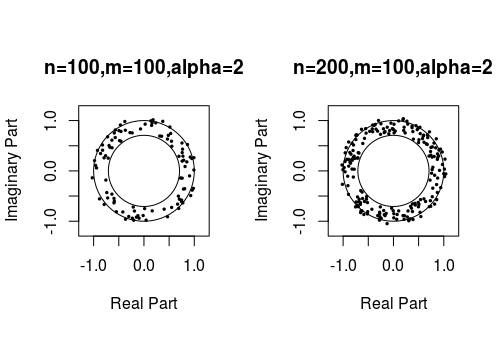
\includegraphics[width=150mm,scale=0.6]{Ring law.png}
    \caption{Graph illustration of the transformed eigenvalues for Ring Law}
    \label{fig:alpha=2}
\end{figure}


%\section*{References}

\bibliographystyle{amsplain}

\begin{thebibliography}{n} %% n is number of items, or the largest label


\bibitem{Handbook of Mathematical Functions}  Abramowitz, M.; Stegun, I.A. (1965): Handbook of Mathematical Functions with Formulas, Graphs, and Mathematical Tables, 9th edn. Dover Publications, New York 
\bibitem{Adhikari}
Adhikari, K.; Reddy, N. K.; Reddy, T. R. and Saha, K. (2016). Determinantal point processes in the plane from products of random matrices. Ann. Inst. H. Poincare Probab. Statist. 52 (1), 16-46.
\bibitem{Bai}Bai, Z.D. (1997). "Circular law". Annals of Probability. 25 (1): 494-529

\bibitem{Dyson}Dyson, F.J. (1962). The three fold way: Algebraic structure of symmetry groups and ensembles in quantum mechanics ,Journal of Mathematical Physics 3,1200-1215.
\bibitem{Ginibre} Ginibre, J. (1965). Statistical ensembles of complex, quaternion and real matrices, Journal of Mathematical Physics 6,  440-449.
\bibitem{Girko} Girko, V.L. (1984). "The circular law". Teoriya Veroyatnostei i ee Primeneniya. 29 (4): 669-679.

\bibitem{GF-TA}Gotze, F.; Tikhomirov, A. (2010). "The circular law for random matrices". Annals of Probability. 38 (4): 1444-1491.
\bibitem{Ipsen} Ipsen, J.R. (2015). Products of independent Gaussian random matrices. Doctoral Dissertation, Bielefeld University.

\bibitem{2017}
Jiang, T.; Qi, Y. (2017). Spectral radii of large non-Hermitian random matrices. Journal of Theoretical Probability 30(1), 326-364.
\bibitem{JiangQi2019} Jiang, T.; Qi, Y. (2019). Empirical distributions of eigenvalues of product ensembles. Journal of Theoretical Probability 32(1), 353-394.
\bibitem{Pan}Pan, G.; Zhou, W. (2010). "Circular law, extreme singular values and potential theory". J. Multivariate Anal. 101 (3): 645-656.
\bibitem{SRP} Qi, Y.; Xie, M. (2019). Spectral Radii of Products of Random Rectangular Matrices. Journal of Theoretical Probability, https://doi.org/10.1007/s10959-019-00942-9.

\bibitem{RudinComplex}
Rudin, W.: Real and Complex Analysis, 3rd edn. McGraw-Hill, New York (1986).


\bibitem{abs}
Silvia, S. (2004). An absolutely continuous function whose inverse function is not absolutely continuous. Note di Matematica 23, n. 1, 2004,47-49.

\bibitem{Tao}Tao, T.; Vu, V. (2010). appendix by Manjunath Krishnapur. "Random matrices: Universality of ESD and the Circular Law". Annals of Probability. 38 (5): 2023-2065.

\bibitem{wishart}  Wishart, J. (1928). The generalized product moment distribution in samples from a normal multivariate population. Biometrika 20, 35-52.

\bibitem{zeng2016}
Zeng, X. (2016). Eigenvalues distribution for products of independent spherical ensmbles. J. Phys. A: Math. Theor. 49, 235201.
\bibitem{zeng2017}
Zeng, X. (2017). Limiting empirical distribution for eigenvalues of products of random rectangular matrices. Statistics and Probability Letters 126, 33-40.

%\bibitem{2017}Jiang, T.; Qi, Y. (2017). Spectral radii of large non-Hermitian random matrices. Journal of Theoretical Probability 30(1), 326-364.





\end{thebibliography}










\end{document}

%% To be filled in the journal office:

@author:
@affiliation:
@title:
@language: English
@pages:
@classification1:
@classification2:
@keywords:
@abstract:
@filename:
@EOI
